\documentclass[preprint,11pt,authoryear]{elsarticle}

% Reduce margins
\usepackage[a4paper, left=2.5cm, right=2.5cm, top=2cm, bottom=2.5cm]{geometry}

% Core encoding and fonts
\usepackage[utf8]{inputenc}
\usepackage[T1]{fontenc}

% Mathematics
\usepackage{amssymb}
\usepackage{amsmath}
\usepackage{dsfont}
\usepackage{bbm}

% Graphics and tikz
\usepackage{tikz}
\usetikzlibrary{shapes, arrows.meta, positioning, calc, backgrounds, fit, shadows}
\usepackage{xcolor}
\definecolor{charcoal}{RGB}{54, 69, 79}

% Tables
\usepackage{tabularx}
\usepackage{booktabs}
\usepackage{threeparttable}
\usepackage{multirow}
\usepackage{siunitx}

\sisetup{
  table-number-alignment = right,
  input-symbols = {<},
  table-align-text-post = false
}
\usepackage{array}
\usepackage{tabularray}
%\usepackage{accessibility}  

\usepackage{graphicx}
\usepackage{accsupp}
\usepackage[titletoc,title]{appendix}

% Layout and formatting
\usepackage{pdflscape}
\usepackage{afterpage}
\usepackage{placeins}
\usepackage{float}
\pdfminorversion=5
\usepackage{setspace}
\usepackage[most]{tcolorbox}
\usepackage[unicode=true]{hyperref}
% Utility
\newcommand{\jelclass}[1]{%
  \par\medskip
  \noindent\textbf{JEL classification:} #1
  \par\medskip
}
\newcommand{\sym}[1]{\ifmmode^{#1}\else\(^{#1}\)\fi}
% Bibliography style
%\usepackage{natbib}[sort]
\biboptions{sort}
\renewcommand{\arraystretch}{0.85}
\setlength{\tabcolsep}{4pt}
\setlength{\intextsep}{8pt plus 2pt minus 2pt}
\setlength{\floatsep}{8pt plus 2pt minus 2pt}
\setlength{\textfloatsep}{10pt plus 2pt minus 2pt}
\DeclareMathOperator*{\argmin}{arg\,min}
\tolerance=200
\emergencystretch=3em
\hyphenpenalty=1000
\hbadness=3000

% Float placement: reduce white space from deferred floats
\renewcommand{\topfraction}{0.9}
\renewcommand{\bottomfraction}{0.9}
\renewcommand{\textfraction}{0.07}
\renewcommand{\floatpagefraction}{0.8}
\setcounter{topnumber}{3}
\setcounter{bottomnumber}{3}
\setcounter{totalnumber}{5}

\begin{document}

\begin{frontmatter}

\title{Credit, Fundamentals, and the Price--Rent Disconnect\\ in
Australian Housing Markets:
Evidence\\ from Five Capital Cities, 2006--2025}
%\author[1]{Ainura Tursunalieva\footnote{ORCID: 0000-0003-2784-9031}}
%\ead{ainura.tursunalieva@data61.csiro.au}
%
%\author[2]{Ratbek Dzhumashev\footnote{ORCID:0000-0003-2428-2762}}
%\ead{ratbek.dzhumashev@monash.edu}
%\affiliation[1]{organization={CSIRO},
%addressline={Research Way},
%city={Clayton},
%postcode={3168},
%state={VIC},
%country={Australia}}
%
%\affiliation[2]{organization={Monash University},
%addressline={Wellington Road},
%city={Clayton},
%postcode={3168},
%state={VIC},
%country={Australia}}

\begin{abstract}
We document a structural change in how dwelling prices and rents are
determined across Australia's five largest capital-city markets, and
characterise how a common credit impulse reaches each. Using quarterly
data for
2006:Q3--2025:Q4, we estimate two reduced-form equations on the
within-city time dimension: a rent equation and a price equation.
Rents are well explained by market fundamentals throughout the
sample, namely a migration-to-completions tightness measure, real wages, and
employment, and this fundamentals structure remains the operative one
throughout, though the relative weight of its channels shifts over time,
with the employment channel strengthening in the second half of the
sample. The price
equation tells a different story. Investor mortgage demand comoves far
more tightly with dwelling prices than with rents, and after 2017 this
asymmetry widens. Because investor credit and prices are partly
determined within the same quarter, we bound the relationship: the
contemporaneous association is large, and it attenuates but does not
vanish when credit is entered as predetermined. Panel local
projections resolve the timing: a credit innovation is capitalised
into prices on impact and reaches rents only with a lag of more than a
year, so the two responses converge over a three-year horizon. The
decoupling is thus a difference in transmission speed and a medium-run
wedge rather than a permanent insulation of rents from financial
conditions. The pattern is broad-based across all five capitals rather
than concentrated in any single city. We interpret the breakdown of the
price--rent relationship as the two markets coming to be governed by
different forces: rents by local housing fundamentals, prices
increasingly by the cost and availability of investor finance. This has
a direct policy implication. Because the two sides of the market respond
to different drivers on different timescales, an instrument calibrated to
one side, a rental-affordability measure acting on a demand side still
anchored to fundamentals, is poorly aligned with a price side that
responds to financial conditions; the rent consequences of a
credit-driven price boom, in particular, materialise only after a delay.
We document this separation rather than estimate the effect of any single
policy, and our extended panel does not support a reading in which
identical national policy produces a financialization gradient across
cities.
\end{abstract}

\begin{keyword}
Regional development \sep Housing financialization \sep Rental markets
\sep Price--rent disconnect \sep Investor credit \sep
Negative gearing \sep Local projections
\end{keyword}

\tnotetext[1]{\textbf{JEL classification:} R21, R23, R28, R31, H53, C23}

\end{frontmatter}

\section{Introduction}
\label{sec:introduction}

Regional development theory has long emphasized the coordination of
economic growth, employment, and social equity within specific
territorial contexts \citep{kuklinski1970regional}, assuming that
market mechanisms would align investment with regional needs through
price signals and competition. The financialization of urban economies
has disrupted these assumptions, introducing distortions beyond the
reach of traditional policy coordination
\citep{fernandez2016financialization, pike2019financialising}.

Nowhere is this disruption more visible than in rental markets.
Across Australia's major cities, between 30\% and 51\% of renters
spend more than 30\% of their income on rent, with the most
financialized markets recording the highest stress rates.
This reflects a global pattern in which market deregulation has
produced rental housing that is costly, insecure, and often
substandard \citep{mckee2017generation, waldron2023generation, bricocoli2024city},
ultimately undermining regional economic competitiveness by pricing
out essential workers.

The underlying driver is the transformation of housing from shelter
into financial asset \citep{stephens2024role}, fuelled by mortgage
expansion and tax incentives such as negative gearing \citep{vidal2024accommodating}.
When investors prioritise capital gains over rental income, the
traditional supply--price relationship weakens and policy
effectiveness erodes \citep{hulse2020everyman}. Housing supply may
increase yet rental security deteriorate, as short-term leases, rent
hikes, and asset speculation displace the provision function
\citep{fields2017unwilling, aalbers2021death}.

Yet a critical gap remains: the extent to which these dynamics vary
\textit{across} metropolitan markets within a single national system.
Existing evidence draws almost entirely on single-city case studies,
leaving unanswered whether financialization produces a uniform
national distortion or a gradient of outcomes that depends on local
investor concentration, institutional structures, and geographic
constraints. Answering this question requires comparative
metropolitan analysis within a shared policy environment.

Australia's five largest state capital cities provide an ideal setting
for this investigation. They share a common national policy framework,
including monetary policy, negative gearing, and migration settings,
but differ substantially in investor concentration, geographic
constraints, and migration exposure. Sydney and Melbourne, the most
heavily invested markets, face severe geographic limitations and high
investor concentration; Brisbane and Perth represent rapid-growth
markets with distinct housing cycles; Adelaide offers a less
constrained comparator with lower investor penetration. These shared
national settings, with differing local conditions, make the five
capitals a natural panel in which to ask how rent and price
determination evolved over time within each market.

Three features make this setting particularly relevant. First,
Australia's negative gearing system fosters a distinctive investor
landscape, which \citet{hulse2020everyman} characterizes as ``mum and
dad'' financialization, setting it apart from institutional models in
other countries. Second, the federal structure generates multi-scalar policy
interactions, with national monetary and tax settings intersecting
state-level housing reforms. Third, the 2017 NSW Housing Affordability
Package provides a concrete, dateable institutional event: announced in
December 2016, the package expanded community housing by 40.7\% while
reducing public housing by 7.0\%, restructuring the institutional
delivery of social housing in Australia's most financialized market.
It gives a specific break date around which to ask whether the
determinants of prices and rents changed; we treat it as one marker
within a longer shift rather than as a treatment whose causal effect we
estimate (Section~\ref{sec:data}).

\paragraph{\bf Research Questions and Approach}
We ask a structural question rather than a policy-evaluation one. What
drives rents, and what drives prices, in these five markets; and did
those drivers change over our sample? Specifically:
(1)~Are rents and dwelling prices governed by the same forces, or by
different ones? (2)~Did the determinants of either shift around the
mid-2010s, when the 2017 NSW package was introduced and investor
activity in housing intensified nationally? (3)~If prices and rents
decoupled, is that because one of them migrated onto a distinct set of
drivers?

Our empirical strategy places inferential weight where a five-city
quarterly panel can bear it: on the within-city time dimension, which
contains roughly seventy quarters of variation per market, rather than
on the thin five-unit cross-section. We estimate two reduced-form
equations. A rent equation relates rent growth to a market-tightness
fundamental (net migration relative to dwelling completions), real
wages, and employment. A price equation relates price growth to the
cost of capital (the cash rate) and investor mortgage demand, alongside
the same fundamentals. We then test whether the financial driver in
each equation changed after 2017 by interacting investor credit with a
post-2017 indicator, and we trace the timing with a rolling-window
decomposition of the share of variation each equation attributes to
investor demand. The design is descriptive: each equation is a standard
reduced form, and we make no claim to identify the causal effect of any
single policy. This is deliberate. It answers the natural ``correlation,
not causation'' objection by not overclaiming causation, and it
identifies the result off the dimension of the data that is actually
informative.

\paragraph{\bf Contributions}
This paper makes three contributions. First, we show that rents and
dwelling prices in these markets are governed by different forces:
rents track local fundamentals (market tightness, real wages, and
employment) throughout the sample, holding across cities, while prices respond
to the cost of capital and to investor credit. The breakdown of the
historical price--rent relationship follows directly from this, rather
than being an unexplained correlation.

Second, we characterise the differing role of investor credit in the
two markets, and we are careful about what the comparison can bear.
Investor credit comoves far more tightly with prices than with rents,
and this asymmetry widens after 2017. Because credit and prices are
partly co-determined within the quarter, we bound the relationship
rather than report a single elasticity: the contemporaneous association
is large, and it attenuates but does not vanish when credit is entered
as predetermined. The rent equation serves as a placebo; if the
price--credit association were a pure artifact of joint determination,
the same force would not so largely spare rents.

Third, we characterise the timing of the contrast using panel
local projections. A credit innovation is capitalised into prices on
impact, consistent with an asset-pricing channel, and reaches rents
only with a lag of more than a year, at the slower speed of occupancy
and supply; over a three-year horizon the two responses converge. The
disconnect is therefore a difference in transmission speed and a
medium-run wedge rather than a permanent insulation of rents from
financial conditions. We further show the pattern is present across
the five capitals and not concentrated in Sydney, the city targeted
by the 2017 package, and that its sharpest movements are centred on the
pandemic period, so we treat the 2017 reform as one marker within a
longer structural shift rather than as its cause. A genuinely
powered cross-sectional test of a financialization gradient would require
sub-metropolitan data, which we flag as a natural extension.

The remainder of the paper proceeds as follows.
Section~\ref{sec:lit} reviews the literature;
Section~\ref{sec:materials_methods} describes data and methods;
Section~\ref{sec:results} presents results;
Section~\ref{sec:discussion} discusses implications; and
Section~\ref{sec:conclusion} concludes.

\section{Literature and Theoretical Background}
\label{sec:lit}

The paper sits within housing economics and draws on three economic
literatures, the user-cost theory of house prices, the supply-constraint
and monetary-transmission literatures, and the migration--housing nexus,
before turning to the financialization literature that describes the
phenomenon we explain. We position the contribution against the economics
of housing first, and treat the broader financialization account as the
description of the decoupling whose mechanism we identify.

The organising idea is the standard one in housing economics: a dwelling
is at once a consumption good, whose rent is the price of housing
services, and an asset, whose price is the present value of those services
and of expected capital gains. In the user-cost framework the two are
linked through the cost of capital, so that prices and rents move together
when both respond to broad housing demand and can diverge when the
asset side loads on financial conditions that the service side does not.
This is the link our estimation tests directly, by asking whether prices
and rents have come to load on different drivers. The cointegration
literature on housing provides the time-series counterpart, treating rents
and prices as potentially I(1) series whose long-run relationship can
weaken \citep{kenny1999modelling}; we take the question of whether that
relationship has broken down to the within-city panel.

On the supply side, \citet{glaeser2003impact} established that regulatory
and geographic constraints shape regional housing supply, but more recent
work finds that financial factors increasingly dominate the supply
response. \citet{greenaway2023impact} show that Auckland's land-use
deregulation yielded minimal affordability gains because investor demand,
driven by capital-gains expectations rather than rental yields, absorbed
the new supply, and \citet{egan2023regime} identify regime shifts in which
the traditional supply--demand relationship breaks down, so that
interventions premised on classical market assumptions can fail precisely
when they are most needed. These findings motivate a design in which the
price response to investor finance is allowed to differ from the rent
response to fundamentals rather than being constrained to move with it.

The assumption of uniform national policy effects is itself challenged by
evidence of regionally differentiated monetary transmission.
\citet{koeniger2022transmission} document how institutional differences
across European regions cause identical central-bank actions to produce
divergent housing outcomes, and \citet{calza2013housing} show that
monetary policy disproportionately affects regions with more volatile
employment. In Australia, \citet{graham2023house} find that interest-rate
changes affect metropolitan and regional markets very differently. A
recognised gap, noted by \citet{stephens2024role}, is that this literature
has concentrated on homeownership and the mortgage channel and has
relatively little to say about rental-market dynamics specifically
\citep{KUANG2026105191}, even as rental housing accommodates a growing
share of urban populations. Separating the rent and price equations and
tracing how a common credit impulse reaches each is one way to address
that gap.

Migration enters as a demand fundamental on the rent side, and the
economics literature here is uneven. Work on immigration and house prices
is well developed \citep{saiz2010geographic, sanchis2023decomposing}, but
the effect on rents is less studied despite renters' over-representation
among recent migrants \citep{nygaard2011international}.
\citet{sharpe2019reevaluating} attribute a substantial share of US rental
price variation to immigration, and \citet{moallemi2020impact} find that
immigration effects on Australian rents vary across cities, with Sydney
most exposed. \citet{li2024internal} add that housing costs themselves
drive internal migration in Australia, so that constrained markets export
population to less constrained ones, a sorting channel through which rents
feed back into the regional distribution of labour
\citep{haas2014commuting}. We capture the demand side of this nexus
through a market-tightness measure, net migration relative to dwelling
completions, rather than through migration alone.

Against this economic background, a large literature documents the
transformation of housing from shelter into financial asset
\citep{fernandez2016financialization, aalbers2021death} and the resulting
decoupling of prices from rents. The form of this process is known to
vary with local institutions \citep{christophers2015limits}; in Australia
\citet{hulse2020everyman} describe a distinctive small-investor
financialization driven by negative gearing. This literature establishes
the phenomenon, prices pulling away from rents, but typically leaves the
decoupling as a documented correlation rather than a mechanism. We take it
in a different direction. Rather than asking whether the degree of
financialization varies across markets, we ask whether it drives a wedge
\emph{within} a market, between the determinants of prices and the
determinants of rents, and we trace how a common financial impulse
reaches each outcome. This reframes the decoupling as the mechanical
consequence of the two outcomes loading on different drivers, which the
within-city panel can test.

\label{sec:comparative_lit}
Two features distinguish our design from this prior work. First, the
within-market question, whether the determinants of rents and prices
diverge over time, has not been posed: \citet{moallemi2020impact} compare
migration--rent dynamics across the Australian capitals but do not examine
the broader transmission channels or the divergence of price and rent
determination. Second, identifying that divergence requires a common
policy environment with within-market time variation rather than a
single-city study, which \citet{koeniger2022transmission} show is the
informative dimension for separating systematic transmission from
city-specific idiosyncrasy. The five Australian capitals provide exactly
this setting.

Our contribution synthesises these literatures. Estimating separate rent
and price equations on the within-city time dimension across five
Australian metropolitan markets, we show that the two outcomes come to be
governed by different forces, fundamentals for rents and investor finance
for prices, and we trace the dynamic mechanism, fast capitalisation into
prices and slow transmission to rents, that produces the breakdown of the
price--rent relationship.

\section{Methods}
\label{sec:materials_methods}

\subsection{Conceptual Framework}
\label{sec:theory}

Our starting point is that a dwelling is two things at once: a place to
live, whose rent is the price of a housing service, and an asset, whose
price is a claim on future housing services and capital gains. When both
are governed by the same broad housing demand, rents and prices move
together, which is the historical norm in these markets. They can come
apart if the two outcomes begin to load on different drivers, with rents
tracking the fundamentals of the service market while prices track the
conditions of asset finance. Documenting whether and when that happens,
and characterising how a common financial impulse reaches each outcome,
is the object of the paper.

This framing yields a small set of expectations that map directly onto
the estimation, without requiring us to take a full structural model to
the data. We set the underlying supply-and-demand system, including the
crowding-out term, the rental-demand split between traditional and
finance-driven components, and a policy-misalignment condition, in
Appendix~\ref{sec:model}; here we carry only what motivates the two
estimating equations and the reduced form they specialise.

The reduced-form rental price equation for city $j$ is
\begin{equation}
\label{eq:reduced_regional}
R_{jt} = F(C_{j,t-1},\; r_{t-1},\; CO_{j,t-1},\;
P_{j,t-1},\; M_{j,t-1},\; w_{j,t-1},\;
N_{j,t-1},\; S^G_{jt},\; NH_{jt}),
\end{equation}
a function of construction costs, the national interest rate, a
crowding-out term capturing competition for construction capacity,
lagged property prices, migration, wages and employment, public housing
supply, and owner-occupier demand. The price equation is the asset-side
counterpart, in which the cost of capital and investor mortgage demand
enter directly. The estimation retains the parsimonious subset of each
that a within-city first-difference design can identify, which we set out
in Section~\ref{sec:methods}.

Four expectations follow. First, rents are governed by service-market
fundamentals, the balance of migration against new dwelling supply
(market tightness), wages, and employment, and this set should remain the
governing one throughout the sample and hold city by city, even if the
relative weight on each channel shifts over time. Second, dwelling prices
are governed by the cost of capital and by investor mortgage demand, with
at most a secondary role for the rental fundamentals. Third, the loadings
of the two outcomes on investor finance should move apart over the sample:
after the mid-2010s prices should load more heavily on investor credit
while rents should not, which is what produces the observed disconnect.
Fourth, because prices capitalise financial conditions quickly while rents
adjust through slower occupancy and supply channels, the two should differ
in the speed with which an investor-credit innovation reaches them,
converging only over the medium run. We do not advance a cross-city
financialization gradient as an expectation: with five units it cannot be
identified, and we treat any cross-city differences descriptively. We use
the pre-2017 property--rental correlations, near-uniform across the
capitals (range 0.941--0.979), only to note that the two markets began the
sample closely integrated everywhere, not as a cross-sectional moderator.

Figure~\ref{fig:transmission} organises these channels into a rent side
tied to fundamentals and a price side tied to investor finance, the
separation of which the estimation then tests in the time dimension.
Federal settings (monetary policy, negative gearing, migration) shape
structural conditions and interact with state-level reforms through
market dynamics rather than explicit coordination; the 2017 NSW package
enters as one dateable marker within that environment rather than as a
treatment whose effect we estimate.

\begin{figure}[!htp]
\centering
\BeginAccSupp{method=pdfstringdef,unicode,Alt={Three-zone transmission diagram. Left, the price side (asset finance): monetary policy sets interest rates, while negative gearing and investor credit feed prices, with investor credit the main channel that strengthens after 2017. Middle, a shared investment and construction band: interest rates feed private investment (the cost-of-capital channel); private investment both raises prices directly and builds construction capacity, which produces dwelling completions; public investment competes for capacity (crowding out). Right, the rent side (service fundamentals): completions form the denominator and migration the numerator of market tightness, which together with wages and employment drives rents. A dotted arrow carries the slow, lagged transmission from prices to rents; both outcomes feed a terminal price-rent disconnect. An edge key distinguishes main, secondary, sign-ambiguous, crowding-out, and slow or weak channels.}}
{%
\definecolor{priceLine}{HTML}{8C2D3A}\definecolor{priceNode}{HTML}{E8B4BB}%
\definecolor{priceFill}{HTML}{F3E3E5}\definecolor{rentLine}{HTML}{2A7F77}%
\definecolor{rentFill}{HTML}{E2F0EE}\definecolor{rentNode}{HTML}{A8D5CE}%
\definecolor{slate}{HTML}{5B6770}\definecolor{slateFill}{HTML}{EEF1F2}%
\definecolor{termFill}{HTML}{2C3E50}\definecolor{amber}{HTML}{C99A2E}%
\definecolor{rust}{HTML}{B5651D}\definecolor{figink}{HTML}{1F2A30}%
\resizebox{\linewidth}{!}{%
\begin{tikzpicture}[
  font=\small,
  >={Stealth[length=2.2mm]},
  box/.style={rounded corners=3pt, draw=slate, fill=slateFill, line width=0.9pt,
              align=center, inner sep=4pt, text=figink, minimum height=9mm, minimum width=26mm},
  core/.style={rounded corners=4pt, line width=1.5pt, align=center, inner sep=5pt,
               text=figink, minimum width=26mm, minimum height=13mm, font=\bfseries\large},
  term/.style={rounded corners=4pt, draw=figink, fill=termFill, text=white, line width=1.4pt,
               align=center, inner sep=6pt},
  main/.style={line width=2.0pt},
  sec/.style={line width=1.1pt},
  weak/.style={line width=1.1pt, dotted},
  amb/.style={line width=1.1pt, dashed, draw=amber},
  crowd/.style={line width=1.1pt, dashed, draw=rust},
  lbl/.style={font=\scriptsize, fill=white, inner sep=1.5pt},
]
\node[box, draw=priceLine, fill=priceFill, line width=1.3pt, text width=34mm, minimum height=22mm] (fin) at (0,0)
  {\textbf{Finance conditions}\\[3pt]\footnotesize Monetary policy $\to$ rates\\ Investor credit\\ Negative gearing};
\node[core, draw=priceLine, fill=priceNode] (prices) at (6.8,1.7) {PRICES};
\node[core, draw=rentLine, fill=rentNode]  (rents)  at (6.8,-1.7) {RENTS};
\node[box] (priv)   at (13.0, 1.8) {Private\\investment};
\node[box] (constr) at (13.0, -0.3) {Construction\\capacity};
\node[box] (compl)  at (13.0,-2.4) {Dwelling\\completions};
\node[box, draw=rentLine, fill=rentFill] (tight) at (13.0,-4.5) {Market tightness\\\footnotesize(migration / completions)};
\node[box] (pub) at (17.4, -0.3) {Public\\investment};
\node[box] (mig) at (17.4,-4.5) {Migration\\policy};
\node[box, draw=rentLine, fill=rentFill] (fund) at (6.8,-4.8) {Rent fundamentals\\\footnotesize(wages, employment)};
\node[term, text width=72mm] (disc) at (6.8,-7.8)
  {\footnotesize\textbf{Price--rent disconnect}\\[1pt] Rents: fundamentals-driven \;\textbullet\; Prices: investor-finance-driven};
\draw[->, main, draw=priceLine] (fin.north east) to[out=35,in=200]
node[lbl, text=priceLine, pos=0.6, yshift=7.5pt]{credit (post-2017)} (prices.west);
\draw[->, sec, draw=priceLine] (fin.north east) to[out=42,in=172]
  node[lbl, text=priceLine, pos=0.2, above=8pt]{cost of capital} (priv.west);
\draw[->, sec, draw=priceLine] (priv.west) to[out=210,in=28]
node[lbl, text=priceLine, pos=0.55, yshift=-9.5pt]{investment} (prices.east);
\draw[->, main, draw=rentLine] (priv) -- (constr);
\draw[->, sec, draw=rentLine] (constr) -- (compl);
\draw[->, sec, draw=rentLine] (compl) -- (tight) node[lbl, text=rentLine, pos=0.5]{denominator};
\draw[->, crowd] (pub.west) -- (constr.east);
\node[lbl, text=rust, anchor=south] at (15.2, -0.18) {crowding out};
\draw[->, amb] (mig.west) -- (tight.east);
\node[lbl, text=amber, anchor=south] at (15.5, -3.98) {$\pm$ migration};
\draw[->, main, draw=rentLine] (tight.west) to[out=178,in=-18]
  node[lbl, text=rentLine, pos=0.6]{significant} (rents.east);
\draw[->, sec, draw=rentLine] (fund.north) -- (rents.south) node[lbl, text=rentLine, pos=0.55]{stable};
\draw[->, weak, draw=priceLine] (prices.south) --
node[lbl, text=priceLine, pos=0.5, xshift=1mm]{slow, lagged} (rents.north);
\draw[->, sec, dashed, draw=priceLine] (prices.west) to[out=200,in=148] (disc.north west);
\draw[->, sec, dashed, draw=rentLine] (rents.south east) to[out=-80,in=40] (disc.north east);
\begin{scope}[on background layer]
  \node[rounded corners=5pt, draw=priceLine, dash pattern=on 3pt off 2pt, line width=0.8pt,
        fit=(fin), inner sep=8pt, label={[priceLine,font=\footnotesize]above:ASSET FINANCE}] {};
  \node[rounded corners=5pt, draw=slate, dash pattern=on 3pt off 2pt, line width=0.8pt,
        fit=(priv)(constr)(compl)(tight)(pub)(mig), inner sep=9pt,
        label={[slate,font=\footnotesize]above:INVESTMENT \& CONSTRUCTION}] {};
  \node[rounded corners=5pt, draw=rentLine, dash pattern=on 3pt off 2pt, line width=0.8pt,
        fit=(prices)(rents)(fund), inner sep=10pt,
        label={[rentLine,font=\footnotesize]above:TRANSMISSION CORE}] {};
\end{scope}
\node[anchor=north, draw=slate!50, rounded corners=3pt, line width=0.6pt,
      inner sep=5pt, font=\scriptsize, align=center] at ($(disc.south)+(0,-5mm)$)
  {\textbf{Edge key}\quad
   \textcolor{figink}{\rule[0.4ex]{6mm}{1.8pt}}~main \quad
   \textcolor{figink}{\rule[0.4ex]{6mm}{0.7pt}}~secondary \quad
   \textcolor{amber}{\rule[0.4ex]{5mm}{0.7pt}}~sign-ambiguous \quad
   \textcolor{rust}{\rule[0.4ex]{5mm}{0.7pt}}~crowding out \quad
   \textcolor{figink}{$\cdots$}~slow / weak};
\end{tikzpicture}%
}%
}
\EndAccSupp{}
\caption{Transmission channels into prices and rents. The asset-finance
channels enter on the left: investor credit, the main channel and the one
that strengthens after 2017, alongside negative gearing and the cost of
capital. The cost-of-capital channel operates through investment, since
monetary policy sets interest rates, which move private investment in the
investment-and-construction band on the right. Private investment is the
hinge between the two sides; it raises prices directly, the fast asset
channel, and it builds construction capacity and hence dwelling
completions, the slow supply channel, with public investment competing for
the same capacity through crowding out. Completions, the denominator, and
migration, the numerator, form market tightness, which together with
wages and employment drives rents through the transmission core in the
middle. A credit impulse thus reaches prices on impact and rents only
slowly, through building and through the dotted price-to-rent link, and
both outcomes feed the price--rent disconnect. Edge weight and style
indicate each channel's role; see the key. The structural model is given
in Appendix~\ref{sec:model}.}
\label{fig:transmission}
\end{figure}

To operationalise these expectations, we specify two reduced-form
equations, one for rents and one for prices, and a test that interacts
investor demand with the post-2017 period, allowing the data to reveal
which channels are active and whether the price--credit relationship
strengthens after the break.

\subsection{Empirical Specification}

Building on the theoretical framework, we estimate a reduced-form
rental price equation (Equation~\ref{eq:reduced_regional}) as an
autoregressive distributed lag (ARDL) model for city $j$:

\begin{equation}
\label{eq:empirical}
R_{jt} = \beta_{0j} + \alpha_{1j} R_{j,t-1} + \alpha_{2j} \text{POST}_{t}
+ \mathbf{X}_{jt}'\boldsymbol{\beta}_j + \varepsilon_{jt}
\end{equation}

Here, $R_{jt}$ denotes the rental price index in city $j$; $\text{POST}_{t}=\mathds{1}[t\geq 2017\mathrm{:}Q1]$ for all cities.
This is a policy intervention dummy capturing city-specific housing reforms, which, for non-Sydney cities, captures the post-2017 institutional environment broadly, while in Sydney it is related to the public housing reform.
%(equal to 1 from 2017:Q1 onward for Sydney);
 We denote  a Sydney-only NSW-reform indicator as
$D_{jt}^{NSW}=\mathds{1}[j=\text{Sydney}]\cdot \text{POST}_{t}$ and $\mathbf{X}_{jt}$ is a
vector of explanatory variables derived from the theoretical model.
Specifically,
$\mathbf{X}_{jt} = [C_{j,t-1},\; r_{t-1},\; GFCF^{P}_{j,t-1},\;
GFCF^{G}_{j,t-1},\; P_{j,t-1},\; M_{j,t-1},\; w_{j,t-1},\;
N_{j,t-1},\; HHS_{jt}]$. In this specification, $C_{j,t-1}$ refers to
construction costs; $r_{t-1}$ to the lagged cash rate (national);
$P_{j,t-1}$ is the property price index; $M_{j,t-1}$ captures net
migration flows; $w_{j,t-1}$ and $N_{j,t-1}$ denote average wages and
employment; and we proxy  owner-occupier demand, $NH_{jt}$, using household housing services consumption $(HHS_{jt})$.
To model the crowding-out effect, the concurrent competition between
public and private investment for construction capacity, the theoretical
specification includes public and private Gross Fixed Capital Formation
($GFCF^{G}_{j,t-1}$ and $GFCF^{P}_{j,t-1}$) separately rather than using
the crowding-out ratio $CO_{j,t-1}$ directly, which would in principle
allow the data to determine whether the crowding-out mechanism operates
differently across cities with varying geographic constraints. In
estimation we retain the parsimonious specifications below, which drop
the GFCF terms; we return to this reduction where the rent equation is
introduced (Section~\ref{sec:methods}).

We estimate the two reduced-form equations as within-city
first-difference models over 2006:Q3--2025:Q4, with the stationary
tightness measure in levels (lagged) and the $I(1)$ series in
differences. A mean-group estimator allows fully heterogeneous
city-level coefficients in the rent equation, confirming that the
fundamentals relationship holds market by market. Identification rests
on the within-city time dimension rather than the five-unit
cross-section.



\subsection{Data Sources and Description}
\label{sec:data}

Our empirical design uses quarterly data from five Australian capital
cities (Sydney, Melbourne, Brisbane, Adelaide, and Perth) covering
2006:Q3 to 2025:Q4, with most series extending to 2025:Q4 and the
binding endpoint set by the publication lag of net migration. The
within-city time dimension carries the identification: about seventy-eight
quarters of data per market, roughly seventy after differencing and
lagged terms enter the estimation, estimated jointly across the five
capitals. We document below three corrections to the price and flow
series relative to earlier versions of this panel, together with the
construction of a continuous price index after the discontinuation of
the ABS capital-city series in 2021.

The panel window is determined by binding data constraints: capital city
property price indices from the Australian Bureau of Statistics (ABS)
Catalogue 6416.0 begin in 2003:Q3, while quarterly state-level overseas
migration data begin in 2006:Q3. The five cities were selected based
on three criteria: population size (each exceeds one million
residents), data completeness across all variables, and variation in
housing market structure, spanning highly financialized markets
(Sydney, Melbourne), rapid-growth markets (Brisbane, Perth), and a
less constrained benchmark (Adelaide).
\subsubsection{Variable Construction and Sources}

Table~\ref{tab:data_sources} (Appendix) provides full variable
definitions, sources, and geographic coverage. Briefly, outcome variables
are capital-city rental price indices (ABS 6401.0) and residential
property price indices (ABS 6416.0); investment is measured by public and
private Gross Fixed Capital Formation (GFCF; ABS 5220.0 State Accounts);
labour market conditions by employment (ABS 6202.0), wages measured by
the Wage Price Index (WPI; ABS 6345.0), and labour income (ABS 5220.0);
investor mortgage demand by the value of new investor housing loan
commitments by state (ABS Lending Indicators, the dataflow successor to
Catalogue 5601.0 Table 14), with national investor and owner-occupier
housing credit and the net loan-purpose switching flow from the Reserve
Bank's D2 series used in the appendix robustness checks; migration by net
overseas and interstate flows (ABS 3101.0), with net overseas migration
disaggregated by visa-and-citizenship group (ABS Overseas Migration)
employed in the appendix mechanism check; and monetary policy by the cash
rate (RBA). State-level
variables serve as city proxies, appropriate given that each capital city
accounts for 65--79\% of its state's economic activity.

Two features of the outcome series warrant explicit statement. The rent
measure is the housing (rent) component of the ABS Consumer Price Index
(Catalogue 6401.0), an index of rents actually paid rather than a hedonic
or repeat-lease rental price index; it is the longest consistent
capital-city rent series available and is standard in Australian housing
work, but it tracks average rents paid across the stock, not new-lease
asking rents, and we interpret it accordingly. For dwelling prices, the
ABS discontinued its established residential property price index, so we
construct a single continuous capital-city series by splicing: for Sydney
we use the Bank for International Settlements all-dwellings series, and
for the other four capitals we extend the ABS 6416.0 index with the ABS
Total Value of Dwellings mean-price series, chain-linking at the splice
point so that growth rates rather than levels are joined. The splice
affects the level of the index, which city fixed effects and
first-differencing absorb, not the quarter-to-quarter growth that the
estimation uses. Table~\ref{tab:data_sources} lists each underlying
series and its coverage.

\subsubsection{Cross-City Summary Statistics}

Table~\ref{tab:cross_city_summary} presents summary statistics across
the five cities for the panel period (2006:Q3--2025:Q4), describing the
range of housing-market conditions in the panel.

\begin{table}[!htbp]
\centering
\footnotesize
\caption{Cross-City Summary Statistics, 2006:Q3--2025:Q4}
\label{tab:cross_city_summary}
\begin{threeparttable}
\setlength{\tabcolsep}{5pt}
\begin{tabular*}{\textwidth}{@{\extracolsep{\fill}}lccccc@{}}
\toprule
& \textbf{Sydney} & \textbf{Melbourne} & \textbf{Brisbane}
& \textbf{Adelaide} & \textbf{Perth} \\
\midrule
\multicolumn{6}{l}{\textit{Price Dynamics}} \\
Rental Index, mean & 108.6 & 106.8 & 106.0 & 107.5 & 98.9 \\
Property Price Index, mean & 148.3 & 131.0 & 128.5 & 125.2 & 113.7 \\
Prop.--Rent Corr. (pre-2017) & 0.98 & 0.97 & 0.97 & 0.97 & 0.95 \\
Prop.--Rent Corr. (post-2017) & 0.77 & 0.26 & 0.96 & 0.98 & 0.97 \\
Correlation change & $-$0.21 & $-$0.71 & $-$0.01 & $+$0.02 & $+$0.02 \\
\addlinespace
\multicolumn{6}{l}{\textit{Migration (thousands, quarterly mean)}} \\
Net Overseas & 19.9 & 17.7 & 9.9 & 3.6 & 7.5 \\
Net Interstate & $-$5.0 & 0.0 & 4.8 & $-$0.7 & 0.9 \\
\addlinespace
\multicolumn{6}{l}{\textit{Investment (AUD bn, quarterly mean)}} \\
Public GFCF & 7.25 & 5.31 & 5.25 & 1.41 & 2.44 \\
Private GFCF & 25.60 & 21.35 & 18.24 & 5.04 & 15.93 \\
Public/Private ratio & 0.28 & 0.25 & 0.29 & 0.28 & 0.15 \\
\addlinespace
\multicolumn{6}{l}{\textit{Labour Market}} \\
Employment (millions) & 3.81 & 3.10 & 2.45 & 0.84 & 1.34 \\
WPI Index, mean & 123.8 & 124.6 & 124.3 & 124.2 & 124.3 \\
\addlinespace
\multicolumn{6}{l}{\textit{Market Structure}} \\
Post-2017 corr.\ decline$^{b}$ & Small & Large & None
& None & None \\
Geographic constraint$^{c}$ & Severe & Moderate & Low
& Low & Moderate \\
\bottomrule
\end{tabular*}
\begin{tablenotes}[flushleft]
\scriptsize
\item \textit{Notes:} Up to $N = 78$ quarters per city (binding endpoint
2025:Q4). Indices use
2011--12 base. Rolling correlations use a 20-quarter (5-year)
trailing window; pre-2017 and post-2017 values are point-in-time
snapshots from the rolling series (not period averages): specifically,
the rolling correlation at the last quarter before 2017:Q1 and at
2025:Q4 respectively.
$^{b}$Large = post-2017 rolling correlation decline $> 0.30$;
Small = between 0 and $0.30$; None = no decline. Reported descriptively,
not as a financialization-intensity index. $^{c}$Following
\citet{saiz2010geographic}: Severe =
multiple natural barriers; Moderate = partial; Low = unconstrained.
\end{tablenotes}
\end{threeparttable}
\end{table}

Three patterns in Table~\ref{tab:cross_city_summary} describe the
variation in the panel. First, the post-2017 decline in the
property--rental correlation is largest in Sydney and Melbourne and
small or absent in the other capitals; we report this as a descriptive
contrast, not as an identified gradient (Figure~\ref{fig:price_ts}).
Second, migration pressures are unevenly distributed: Sydney and
Melbourne receive large overseas inflows but experience net interstate
outflows, consistent with affordability-driven displacement
\citep{li2024internal}, whereas Brisbane receives both overseas and
interstate migrants. Third, the public-to-private GFCF ratio and
absolute investment magnitudes differ substantially, which is relevant
to whether the crowding-out mechanism operates differently across
capacity-constrained and unconstrained cities.

Table~\ref{tab:est_summary} reports summary statistics for the variables
as they enter the estimation: the $I(1)$ series in quarter-on-quarter
log-differences, market tightness in levels, and the price--rent gap in
log levels. The differenced series are small and roughly symmetric, which
is the behaviour the log-difference transformation is designed to
produce; tightness, a ratio of net migration to completions, is the one
variable with a wider spread, and it takes occasional negative values in
the 2020--21 border-closure quarters when net migration itself turned
negative.

\begin{table}[!htbp]
\centering
\footnotesize
\caption{Summary Statistics for Estimation Variables, 2006:Q3--2025:Q4}
\label{tab:est_summary}
\begin{threeparttable}
\setlength{\tabcolsep}{6pt}
\begin{tabular*}{\textwidth}{@{\extracolsep{\fill}}lrrrrr@{}}
\toprule
Variable & $N$ & Mean & SD & Min & Max \\
\midrule
$\Delta \ln$ Rent              & 385 & 0.008 & 0.009 & $-$0.025 & 0.033 \\
$\Delta \ln$ Price             & 385 & 0.013 & 0.024 & $-$0.057 & 0.092 \\
$\Delta \ln$ Investor credit   & 385 & 0.014 & 0.148 & $-$0.326 & 0.394 \\
$\Delta \ln$ WPI (wages)       & 385 & 0.007 & 0.004 & $-$0.001 & 0.023 \\
$\Delta \ln$ Employment        & 385 & 0.005 & 0.010 & $-$0.066 & 0.043 \\
$\Delta$ Cash rate             & 385 & $-$0.030 & 0.409 & $-$1.887 & 1.393 \\
Tightness (level)              & 370 & 1.430 & 0.931 & $-$1.354 & 5.497 \\
Price--rent gap (log level)    & 390 & 0.172 & 0.169 & $-$0.132 & 0.669 \\
\bottomrule
\end{tabular*}
\begin{tablenotes}[flushleft]
\scriptsize
\item \textit{Notes:} Pooled across the five capitals. $\Delta \ln$
denotes the quarter-on-quarter log-difference (a value of 0.010 is
approximately one percent growth); $\Delta$ Cash rate is the
quarter-on-quarter change in percentage points. Tightness is net
migration over the trailing four quarters relative to dwelling
completions over the same window, entered in levels and lagged one
quarter in estimation; its negative minimum reflects the 2020--21
border-closure quarters in which net migration was negative. The
price--rent gap is the log of the dwelling-price index over the rent
index, entered as a lagged level control. $N$ is the number of
city-quarters available for each variable after differencing and lagging;
tightness loses further observations to its trailing four-quarter
construction and one-quarter lag.
\end{tablenotes}
\end{threeparttable}
\end{table}

\begin{figure}[!htbp]
\centering
\BeginAccSupp{method=pdfstringdef,unicode,Alt={Time series plot of rental price indices for five Australian
capital cities from 2006 to 2025, showing broadly co-moving
trajectories, with Perth declining around 2014 to 2020 with the end of
the mining investment boom. A single dashed line marks 2017 Q1.}}
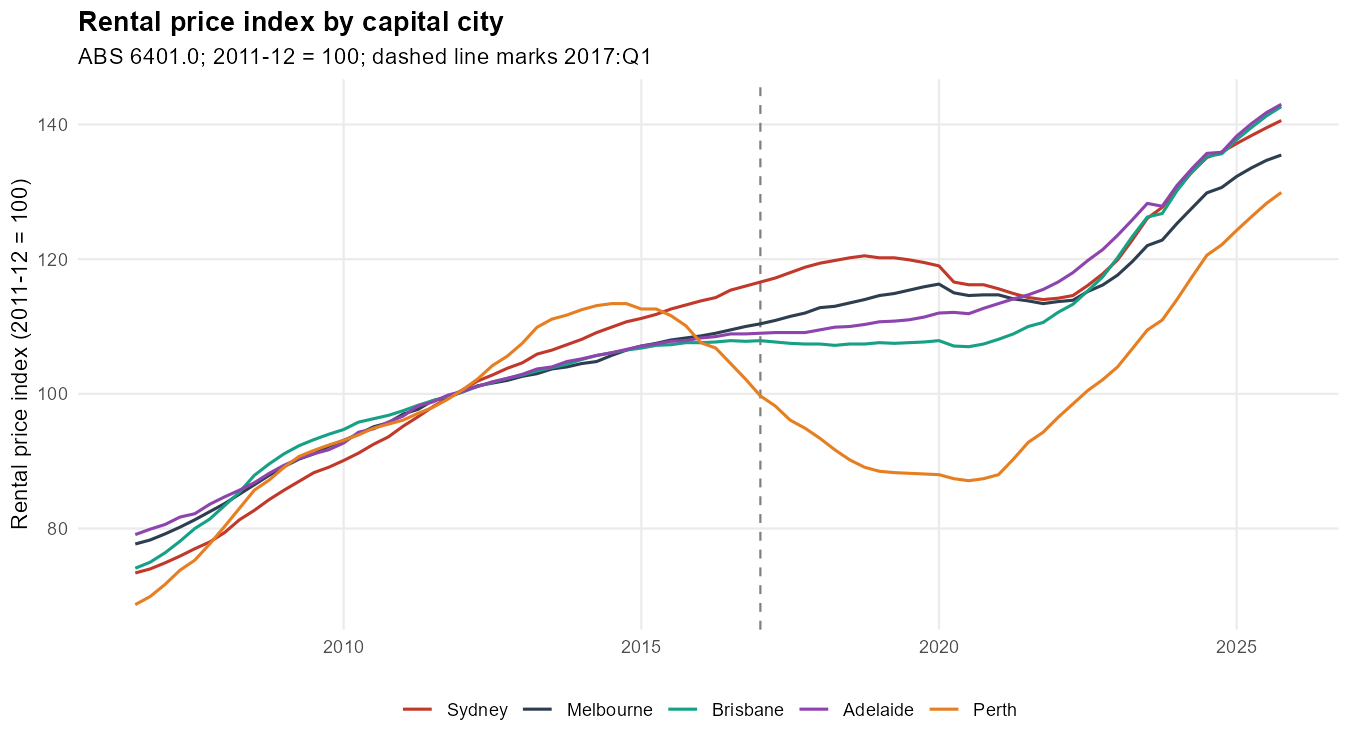
\includegraphics[width=\textwidth,height=0.34\textheight,keepaspectratio]{fig_rental_trajectories.png}
\EndAccSupp{}
\caption{Rental price index trajectories, five Australian capital
cities, 2006:Q3--2025:Q4 (ABS 6401.0; base: 2011--12 = 100). The dashed
line marks 2017:Q1. Perth diverges from $\sim$2014 with the mining
investment cycle. The series move broadly together, consistent with
rents across the capitals being driven by common housing-demand
fundamentals; the figure is descriptive and does not underpin a
treatment-control comparison.}
\label{fig:price_ts}
\end{figure}


Index variables (rents, the wage price index) are expressed on a common
base and are comparable in level across cities, while the level
variables differ substantially with city size. These level differences
are absorbed by city fixed effects and first-differencing, so the
estimation works off within-city changes rather than cross-city levels.
The large cross-city dispersion in property prices, with Sydney highest,
reflects city size and accumulated price growth rather than anything the
design needs to balance.

\subsubsection{The 2017 Break Date}

We set the post-2017 indicator to begin in 2017:Q1, the quarter after
the December 2016 announcement of the NSW package (Section~\ref{sec:introduction}),
fixing the break date from the institutional timeline. The indicator
marks a candidate break in the sample, not a treatment whose effect we
estimate; the analysis tests whether the determinants of prices and
rents change around it.

The rolling price--rent correlation declines after the mid-2010s across
the panel, with the largest declines recorded in Sydney and Melbourne
(Figure~\ref{fig:price_rent_gap}, Section~\ref{sec:descriptive}). The
decline is broad-based rather than specific to Sydney, which is
consistent with common macroeconomic and institutional forces operating
across the metropolitan system rather than with a change confined to one
city. We report these correlation patterns as description only. Our
estimation (Section~\ref{sec:results}) finds the post-2017 strengthening
of the price--investor-credit channel present across the capitals rather
than confined to the most expensive markets; if anything it is weaker in
Sydney. The cross-city differences in the measured magnitude of the
decoupling are therefore not a basis for categorical claims about
differential financialization.

\subsubsection{Data Limitations}

Three limitations warrant acknowledgement. First, state-level variables
serve as proxies for city-level measures for GFCF, labour income, and
housing services consumption. While capital cities dominate their state
economies, this introduces measurement error that may attenuate
estimated coefficients. Second, the panel begins in 2006:Q3,
precluding analysis of pre-GFC financialization dynamics; identification
rests on the within-city time variation over 2006--2025 rather than on
the pre-GFC period. Third, construction cost data at the city level are proxied
using state-level implicit price deflators from the national accounts,
which may not fully capture city-specific cost pressures.

\subsection{Econometric Methods}
\label{sec:methods}

We estimate two reduced-form equations on the five-city quarterly
panel, placing identification on the within-city time dimension. Most
series are $I(1)$ index levels, so we work in first differences; the
market-tightness measure is a ratio of flows and is stationary, so it
enters in levels lagged one quarter. All models include city fixed
effects and use heteroskedasticity- and autocorrelation-robust
(Driscoll--Kraay) standard errors.

Each method below has a specific and limited role, and the set is small
by design. The two reduced-form equations, estimated by within-city
fixed effects, establish what governs rents and what governs prices. The
mean-group estimator checks that the rent relationship holds city by city
rather than only on average. The divergence test, a single interaction of
investor credit with a post-2017 indicator in each equation, asks whether
the price--credit relationship strengthens after the break while the
rent--credit relationship does not. The local projections recover the
timing that the static interaction compresses into one coefficient,
showing how fast a credit innovation reaches prices versus rents. The
shift-share instrument in the appendix is a supplementary check on the
price--credit association, reported as indicative given the small
cross-section, not as the headline. Everything else is robustness. We do
not use the methods to layer additional claims; each addresses one link
in a single argument, from what drives each outcome, to whether the
credit link changes after 2017, to how quickly it transmits.

\paragraph{Stationarity and functional form}
Panel and city-level unit-root tests indicate that log rents, log
prices, log wages, log employment, and log investor commitments are
$I(1)$, consistent with the cointegration literature on housing
\citep{kenny1999modelling}. We therefore difference these series. Market
tightness, net migration over the trailing four quarters relative to
dwelling completions over the same window, is stationary (its
autoregressive root is well below unity), and entering it in levels
rather than differences is both the correct treatment of an $I(0)$
regressor and materially better-fitting: differencing an already
stationary variable over-differences it. The price--rent gap enters the
rent equation in lagged log levels as a level control rather than as an
error-correction term: a residual-based panel test does not find robust
cointegration between log rents and log prices (group-mean ADF
$\approx -1.86$, around the Pedroni five percent critical value), and the
gap carries a coefficient close to zero and statistically insignificant
in every rent specification we estimate, so we do not impose an
error-correction interpretation on it.

The estimated rent equation is a parsimonious reduction of the
theoretical reduced form in Equation~\ref{eq:reduced_regional}. We
retain the terms the within-city first-difference design can identify
and the data support, the tightness fundamental, wages, employment, and
the lagged price--rent gap as a level control, and drop those that enter weakly or are
absorbed by the transformation: construction costs and the cash rate
carry no direct role on the rent side once prices are differenced, the
public and private GFCF terms that proxy crowding-out are a supply-side
channel that the parsimonious rent and price specifications do not
retain, and owner-occupier demand is collinear with the tightness and
price-gap terms. The structural model in Appendix~\ref{sec:model} sets out
the fuller channel set, including crowding-out as competition for
construction capacity; Equations~\ref{eq:rent} and~\ref{eq:price} estimate
the subset that survives, and Figure~\ref{fig:transmission} shows the
thesis those two equations test.

\paragraph{Rent equation}
\begin{equation}
\label{eq:rent}
\Delta r_{it} = \alpha_i + a\,(p-r)_{i,t-1}
 + b_1\,\text{TIGHT}_{i,t-1} + b_2\,\Delta w_{it}
 + b_3\,\Delta n_{it} + \varepsilon_{it},
\end{equation}
where $r$ is log rent, $(p-r)$ the log price--rent gap, $\text{TIGHT}$
market tightness, $w$ log wages, and $n$ log employment. We estimate
Equation~\ref{eq:rent} both as a pooled within (fixed-effects)
estimator and as a mean-group estimator \citep{pesaran1995estimating}
that averages city-specific regressions, the latter confirming that the
fundamentals relationship holds market by market rather than only on
average.

\paragraph{Price equation}
\begin{equation}
\label{eq:price}
\Delta p_{it} = \gamma_i + c_1\,\Delta \text{CASH}_t
 + c_2\,\Delta \iota_{it} + c_3\,\text{TIGHT}_{i,t-1}
 + c_4\,\Delta w_{it} + \eta_{it},
\end{equation}
where $p$ is log price, $\text{CASH}$ the cash rate, and $\iota$ log
investor mortgage commitments.

\paragraph{Divergence test}
The central test interacts investor demand with a post-2017 indicator
$\text{POST}_t$ in both equations:
\begin{equation}
\label{eq:divergence}
\Delta y_{it} = \delta_i + \pi_1\,\Delta \iota_{it}
 + \pi_2\,(\Delta \iota_{it}\!\times\!\text{POST}_t)
 + \mathbf{x}_{it}'\boldsymbol{\psi} + \xi_{it},
\end{equation}
estimated separately with $y = p$ and $y = r$ and the appropriate
controls $\mathbf{x}_{it}$ from Equations~\ref{eq:price}
and~\ref{eq:rent}. The cash rate enters in differences but is not
interacted: across the post-2017 window it is dominated by the COVID
near-zero-rate period and the 2022--23 hiking cycle, making its
interaction a regime artifact rather than a financialization signal; we
report the cash-rate-interacted version as a robustness check. The
parameter of interest is $\pi_2$. A large $\pi_2$ in the price equation
with at most a small $\pi_2$ in the rent equation indicates that
investor credit comoves more tightly with prices than with rents, and
increasingly so after 2017. Because $\Delta\iota_{it}$ and
$\Delta p_{it}$ are partly determined within the quarter, we estimate
Equation~\ref{eq:divergence} both contemporaneously and with investor
credit entered as predetermined (lagged one quarter); the two bracket
the relationship, the contemporaneous estimate as an upper bound that
absorbs simultaneity and the predetermined estimate as a lower bound
that displaces a within-quarter relationship. The rent equation serves
as a placebo for reverse causality. We test $\pi_2 = 0$ in each
equation with a one-degree-of-freedom Wald test, and as a further check
instrument $\Delta\iota_{it}$ with a shift-share instrument
(Appendix~\ref{sec:robustness}), reading the first-stage strength as the
binding diagnostic given the small cross-section.

\paragraph{Local projections}
To recover the dynamics that the static interaction compresses into a
single coefficient, we estimate Jord\`a panel local projections of the
price and rent levels on an investor-credit innovation over horizons
$h = 0,\dots,12$, with city fixed effects and lagged controls that
absorb the predictable component of credit. The impulse is scaled to
one standard deviation of credit growth. Horizon zero retains the
within-quarter simultaneity caveat; horizons from one quarter out are
predetermined and clean of reverse causality. The object of interest is
the difference in the shape and timing of the two response paths.

\section{Results}
\label{sec:results}

We organise the results around the two equations and their divergence.
Section~\ref{sec:identification} states the identification strategy and
its scope. Section~\ref{sec:rent_eq} establishes that rents are
governed by fundamentals, that this holds across cities, and that the
fundamentals remain the operative drivers throughout even as their
relative weights shift over time.
Section~\ref{sec:price_eq} shows that prices respond to the cost of
capital and to investor credit. Section~\ref{sec:divergence} presents
the central contrast and is careful about what it is: a differential
co-movement of investor credit with prices and rents, large
contemporaneously and attenuating but not vanishing once credit is
predetermined. Section~\ref{sec:mechanism} recovers the dynamic
mechanism behind that contrast through local projections, showing that
credit reaches prices fast and rents slowly. Section~\ref{sec:descriptive}
reports the cross-city decoupling as description.

\subsection{Identification and Scope}
\label{sec:identification}

Our design is descriptive reduced-form, and we are explicit about what
it can and cannot deliver. The two equations are standard reduced forms
estimated off roughly seventy quarters of within-city variation, which
is where the statistical power in a five-city panel resides. We do not
claim to identify the causal effect of any single policy on rents; the
2017 NSW package enters as a structural-break date, one event within a
broader shift, not as a treatment whose effect we estimate.
Correspondingly, the cross-city dimension is too thin (five units) to
identify a financialization gradient, and we use it descriptively rather
than as the basis for a typology. This is a deliberate reallocation of
inferential weight onto the part of the data that can bear it: the
changing time-series structure of rent and price determination within
cities, and away from the single-unit and cross-sectional comparisons
that cannot. A genuinely powered cross-sectional test of the
financialization gradient would require sub-metropolitan (SA4/SA3) data;
we flag this as a natural extension rather than attempt it here.

We estimate both equations as within-city (fixed-effects)
first-difference models. The $I(1)$ index series (log rents, log prices,
log wages, log employment, log investor commitments) enter in
differences; the market-tightness measure, a ratio of flows that is
stationary, enters in levels lagged one quarter. Standard errors are
heteroskedasticity- and autocorrelation-robust (Driscoll--Kraay). We report a
mean-group estimator alongside the pooled within estimator for the rent
equation to confirm that the relationship holds city by city.

\subsection{Rents are governed by fundamentals}
\label{sec:rent_eq}

Table~\ref{tab:rent_eq} reports the rent equation. Rent growth responds strongly
and significantly to the lagged market-tightness ratio, to wage growth, and to
employment growth, and these relationships are stable across cities: the mean-group
estimates, which average city-by-city regressions, recover the same pattern as the
pooled within estimates. The lagged price--rent gap does not enter rent growth in
either specification, with a point estimate close to zero and a $p$-value of 0.67
in the pooled model and 0.18 in the mean-group model. Rents track the fundamentals
that a standard housing-demand account would predict, and they do not chase the
widening gap between prices and rents. This result is robust across every
specification we report below and is the empirical anchor of the paper.

The fundamentals structure is stable across cities, but its internal
weights are not constant over time, and we are explicit about this. A
Chow-style test that interacts all four rent regressors with the
post-2017 indicator rejects coefficient equality
($\chi^2_4 = 18.7$, $p < 0.001$), so the rent equation is not a
fixed-coefficient relationship across the sample. The pattern behind the
rejection is interpretable rather than destabilising: interacting the
fundamentals with a linear time trend, the employment channel
strengthens over the sample (trend interaction $+0.013$, $p = 0.06$, with
the rolling-window employment coefficient rising from near zero in the
early 2010s to about $0.15$ by the 2020s), while the wage and tightness
coefficients remain positive and significant throughout but with a
noisier wage pass-through. The substantive claim is therefore that rents
remain governed by the same service-market fundamentals across the whole
sample, with the relative weight on employment growing as the labour
market tightened; it is not that the coefficients are literally constant.
This evolution does not affect the divergence result, which concerns the
investor-credit channel, not the fundamentals.

\begin{table}[t]
\centering
\begin{threeparttable}
\caption{Housing market equations, 2006:Q3--2025:Q4}
\label{tab:rent_eq}
\begin{tabular*}{\textwidth}{@{\extracolsep{\fill}}l
                S[table-format=-1.3, table-space-text-post={\sym{***}}]
                S[table-format=-1.3, table-space-text-post={\sym{***}}]@{}}
\toprule
 & {(1)} & {(2)} \\
\midrule
\multicolumn{3}{l}{\textit{Panel A. Rent growth equation ($\Delta\ln$ rent)}} \\
 & {FD} & {MG} \\
\cmidrule(lr){2-3}
Price--rent gap$_{t-1}$ & {0.001 (0.002)} & {0.007 (0.005)} \\
Tightness$_{t-1}$       & {0.006\sym{***} (0.001)} & {0.005\sym{***} (0.001)} \\
$\Delta\ln$ WPI         & {0.849\sym{***} (0.165)} & {0.799\sym{***} (0.203)} \\
$\Delta\ln$ Employment  & {0.155\sym{***} (0.039)} & {0.129\sym{***} (0.032)} \\
Observations            & {370} & {370} \\
$R^2$                   & {--} & {0.570} \\
\midrule
\multicolumn{3}{l}{\textit{Panel B. Price growth equation ($\Delta\ln$ price)}} \\
 & {Current ($t$)} & {Lagged ($t-1$)} \\
\cmidrule(lr){2-3}
$\Delta\ln$ Investor credit & {0.072\sym{***} (0.013)} & {0.050\sym{***} (0.013)} \\
$\Delta$ Cash rate          & {0.004 (0.006)}          & {-0.006 (0.004)} \\
Tightness$_{t-1}$           & {0.003 (0.003)}          & {0.004 (0.003)} \\
Observations                & {370}                    & {370} \\
\bottomrule
\end{tabular*}
\begin{tablenotes}[flushleft]\footnotesize
\item \textit{Notes:} Coefficients with Driscoll--Kraay standard errors in
parentheses. City fixed effects are used throughout. FD = first-difference
estimator; MG = mean-group estimator; Current and Lagged denote contemporaneous
and one-quarter-lagged regressors. Dependent variables are $\Delta\ln$ rent
(Panel A) and $\Delta\ln$ price (Panel B); wage growth is excluded from Panel B.
\sym{*}$p<0.10$, \sym{**}$p<0.05$, \sym{***}$p<0.01$.
\end{tablenotes}
\end{threeparttable}
\end{table}

\subsection{Prices respond to investor credit and the cost of capital}
\label{sec:price_eq}

Panel B of Table~\ref{tab:rent_eq} reports the price equation. We exclude wage growth, which
has no direct role in a user-cost price relationship, and we report the regressors
both contemporaneously and lagged one quarter, because investor credit and prices
are plausibly determined within the same quarter. Investor-credit growth enters
positively and significantly in both timings. The cash rate is the clearest case
where timing matters. Entered contemporaneously it takes a small positive
coefficient; entered with a one-quarter lag it turns negative, the
sign a user-cost relationship predicts. We read the positive contemporaneous
association as the familiar endogeneity of a policy rate that is itself raised
during booms, when prices are also rising, and the negative predetermined
coefficient as the better-behaved estimate of how the cost of capital feeds into
prices. We therefore do not interpret the contemporaneous cash-rate coefficient and
treat the lagged specification as the more credible of the two.

\subsection{The divergence, and what it is}
\label{sec:divergence}

The descriptive starting point is that prices pulled away from rents over the
sample, sharply so from 2020. Figure~\ref{fig:price_rent_gap} shows the price--rent
ratio rising in every capital, and Figure~\ref{fig:real_rent} shows real rents,
deflated by wages, moving on a quite different path driven by local conditions
rather than by the price cycle. The question is whether this decoupling reflects
investor credit operating on prices in a way it does not operate on rents.

\begin{figure}[t]
\centering
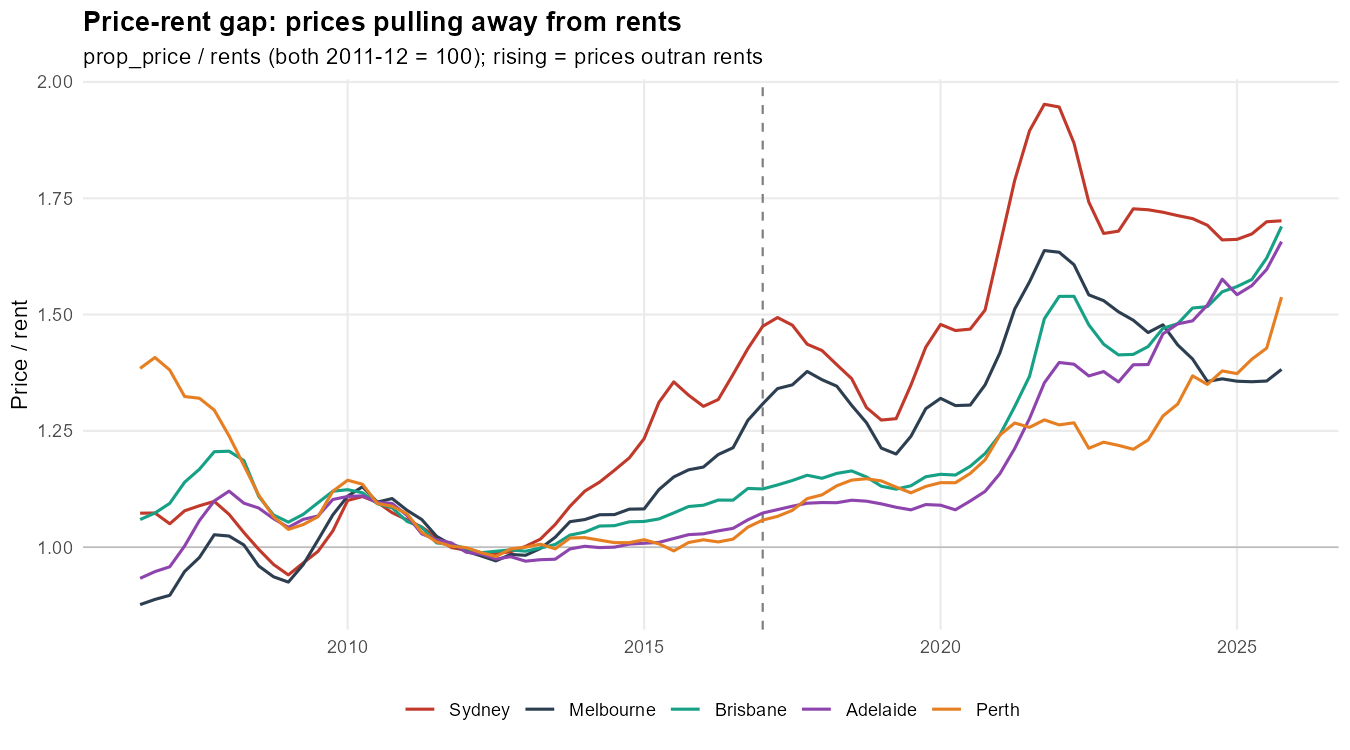
\includegraphics[width=0.8\textwidth]{fig_price_rent_gap.png}
\caption{Price--rent gap by capital city: the dwelling price index over the rent
index (both 2011--12 $=100$). A rising series indicates prices outrunning rents.}
\label{fig:price_rent_gap}
\end{figure}

\begin{figure}[t]
\centering
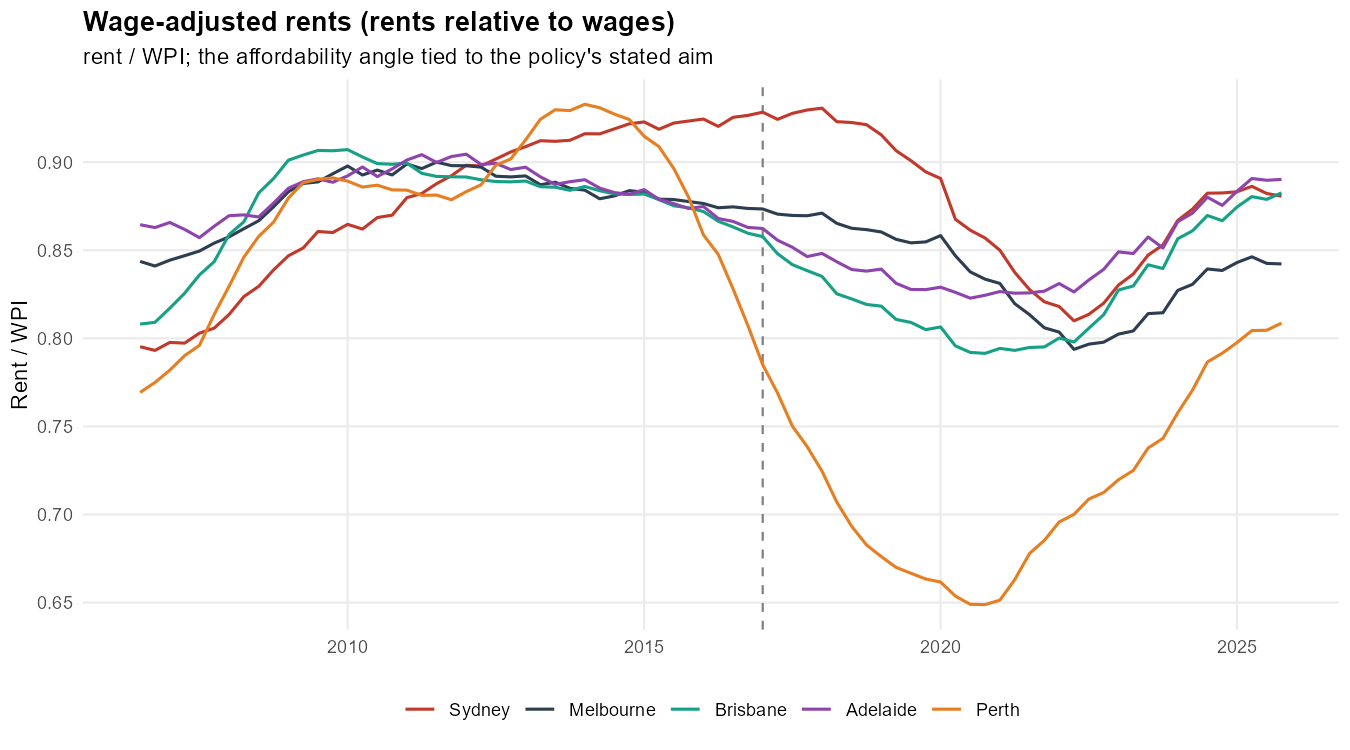
\includegraphics[width=0.8\textwidth]{fig_real_rent.png}
\caption{Real rents, rents deflated by the state wage price index, by capital
city. Broadly stable-to-declining until the pandemic, then recovering, with
Perth's mining-cycle collapse and rebound the main exception.}
\label{fig:real_rent}
\end{figure}

Contemporaneously the contrast is stark. Interacting investor-credit growth with a
post-2017 indicator, the interaction in the price equation is 0.056 ($p<0.01$)
while the same interaction in the rent equation is 0.004 and is not statistically
significant ($p=0.64$), an order of magnitude smaller. Taken at face value
this says that after 2017 investor credit became a far stronger correlate of price
growth than of rent growth.

We do not take it fully at face value, because contemporaneous investor credit and
prices are jointly determined: credit is drawn as purchases settle, so a
within-quarter association partly reflects prices acting on credit as much as credit
acting on prices. To gauge how much of the contrast is co-movement of this kind,
Table~\ref{tab:divergence} re-estimates the interaction with investor credit entered
as predetermined, lagged one quarter. Under predetermination the price interaction
is 0.041 ($p<0.10$) while the rent interaction rises to 0.017 and is significant
($p<0.01$). The two interactions, an order of magnitude apart contemporaneously,
converge under predetermination to within roughly a factor of two and a half, as
the rent response emerges once credit is lagged.

\begin{table}[t]
\centering
\begin{threeparttable}
\caption{Investor credit $\times$ post-2017 interaction, price versus rent}
\label{tab:divergence}
\begin{tabular*}{\textwidth}{@{\extracolsep{\fill}}l
                S[table-format=-1.3, table-space-text-post={\sym{***}}]
                S[table-format=-1.3, table-space-text-post={\sym{***}}]@{}}
\toprule
 & {Price equation} & {Rent equation} \\
\midrule
\multicolumn{3}{l}{\emph{Panel A. Contemporaneous credit}} \\
$\Delta\ln$ Investor credit $\times$ post & {0.056\sym{***} (0.021)} & {0.004 (0.008)} \\
\addlinespace
\multicolumn{3}{l}{\emph{Panel B. Predetermined credit (lagged one quarter)}} \\
$\Delta\ln$ Investor credit$_{t-1}\times$ post & {0.041\sym{*} (0.023)} & {0.017\sym{***} (0.006)} \\
\bottomrule
\end{tabular*}
\begin{tablenotes}\footnotesize
\item Each cell is the interaction coefficient from the equation in
Table~\ref{tab:rent_eq} augmented with the interaction. City
fixed effects; Driscoll--Kraay standard errors in parentheses. \sym{*}$p<0.10$, \sym{**}$p<0.05$,
\sym{***}$p<0.01$.
\end{tablenotes}
\end{threeparttable}
\end{table}

The reading we adopt is therefore deliberately modest. Investor credit comoves more
tightly with prices than with rents, and that asymmetry is large in the same quarter
and attenuates, without vanishing, when credit is predetermined. Neither estimate is
a structural causal elasticity: the contemporaneous figure overstates the role of
credit through simultaneity, and the strictly lagged figure understates it by
displacing a relationship that operates largely within the quarter. What survives
both is a differential co-movement, prices tracking investor credit more closely
than rents do, rather than evidence that credit causally drives prices and leaves
rents untouched. The rent equation functions here as a placebo: if the price--credit
association were a pure accounting artefact of joint determination, the same force
would not so largely spare rents, and the persistence of a small but real
credit--rent association under predetermination is consistent with credit affecting
rents through a slower, supply-side channel.

We further probe the robustness of the price--credit association in two ways
(Appendix~\ref{sec:robustness}). First, we instrument investor-credit growth with a
shift-share (Bartik) instrument formed from each city's pre-2017 investor-credit
weight and leave-one-out national credit growth; with only five cross-sectional
units the first-stage strength is the binding diagnostic, and we report the IV as
indicative rather than as the headline. Second, we confirm that the same instrument
does not load on rents, the placebo direction. The qualitative contrast survives,
but we lean on the predetermined-regressor and local-projection evidence rather than
on the IV.

\subsection{The mechanism: investor credit reaches prices fast and rents slowly}
\label{sec:mechanism}

To recover the timing that the static interactions in Table~\ref{tab:divergence}
compress into a single coefficient, we estimate panel local projections of the price
and rent levels on an investor-credit innovation over twelve quarters, with city
fixed effects and lagged controls that absorb the predictable component of credit.
Figure~\ref{fig:lp} plots the cumulative response of each log level to a
one-standard-deviation credit innovation, with ninety percent Driscoll--Kraay bands.
Horizon zero retains the within-quarter simultaneity noted above; horizons from one
quarter out are predetermined and so are clean of reverse causality from prices back
to credit. The long-horizon estimates are less precise and their windows overlap the
pandemic, so we read the figure for its timing rather than for the exact magnitude
at distant horizons.

The two responses differ in speed, not in whether credit reaches them. Prices
respond on impact, by about 1.2 percent (0.012 log points), build to roughly
2.9 percent (0.029 log points) by the fourth quarter, and remain elevated through
the third year, drifting up to about 3.9 percent (0.039 log points) by the twelfth,
with a shallow mid-window
dip that lies within the bands. Rents are flat and
indistinguishable from zero through the first year, then climb steadily to
about 2.3 percent (0.023 log points) by the twelfth quarter. The horizon
at which the rent response first becomes significant is sensitive to the
number of control lags, falling between the second and the seventh quarter
depending on that choice, so we treat it as approximate; what is stable
across lag specifications is the shape, a delayed rent response that builds
over the second and third years, and the twelfth-quarter magnitude of about
0.02 log points. Credit is capitalised into prices almost at once, as an asset-pricing
channel implies, and reaches rents only with a lag of around a year or more, at the
slower speed of occupancy and supply.

This shape reconciles the static estimates. The contemporaneous interaction reads
the impact horizon, where the price response dwarfs the rent response, while the
predetermined interaction reads a later horizon, where rents have begun to respond,
which is why its rent coefficient is non-zero. Both describe the same paths at
different points rather than conflicting results.

Over the full horizon the rent response closes much of the gap with the price
response. By twelve quarters the point estimates have narrowed and the confidence
bands overlap substantially, so the two responses are no longer statistically
distinguishable, though the price response is itself imprecisely estimated that far
out. The decoupling documented above is therefore a difference in transmission speed
and a medium-run wedge, not a permanent insulation of rents from financial
conditions: a credit impulse that lifts prices on impact works through to rents over
one to three years. The persistent gap in the descriptive series reflects sustained
financial conditions and price-specific drivers such as the cost of capital, rather
than rents never responding, and the lag carries a direct affordability implication,
since the rent consequences of a credit-driven price boom materialise only after a
delay of a year or more.

\begin{figure}[t]
\centering
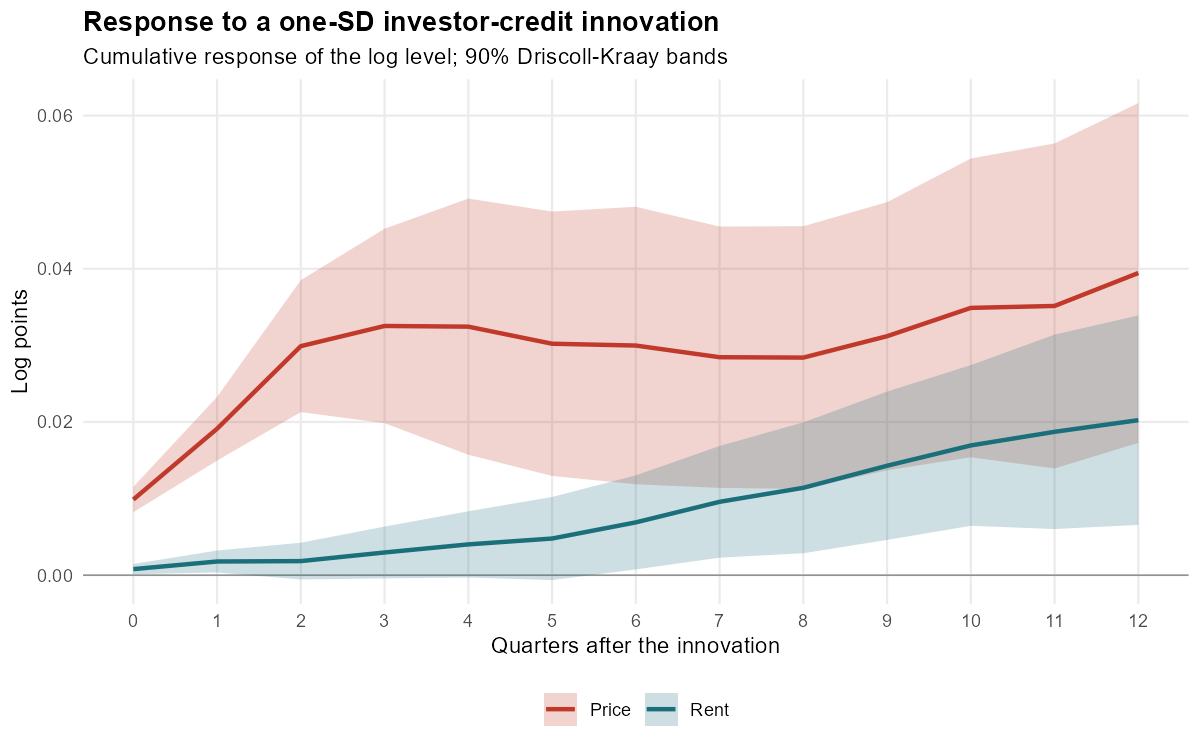
\includegraphics[width=0.8\textwidth]{local_projection_irf.png}
\caption{Cumulative response of the price level and the rent level to a
one-standard-deviation investor-credit innovation, over twelve quarters, in log
points (a response of 0.030 is about 3.0 percent). Panel local projections with
city fixed effects and lagged controls; ninety percent Driscoll--Kraay bands.
Horizon zero carries the within-quarter simultaneity caveat; horizons from one
quarter out are predetermined, and the long-horizon estimates are less precise.}
\label{fig:lp}
\end{figure}

\subsection{The decoupling across cities}
\label{sec:descriptive}

The price--rent ratio rose across all five capitals from near parity in the early
2010s to between $1.4$ and $2.0$ by 2025, most in Sydney
(Figure~\ref{fig:price_rent_gap}). Real rents (rents deflated by wages) were broadly
stable-to-declining until the pandemic and then recovered, with Perth the notable
exception (a sharp mining-cycle rent collapse and rebound), consistent with rents
responding to local fundamentals (Figure~\ref{fig:real_rent}). We report the
cross-city correlation patterns as description only and do not build a
cross-sectional gradient on them. The structural
break in the investor-credit channel dates to 2017, while its largest movements
are concentrated in the pandemic period, so we treat the 2017 package as one
marker within a longer structural shift rather than as its cause: the break
precedes the pandemic, and the pandemic amplifies it.

\section{Discussion}
\label{sec:discussion}

We interpret the results for housing economics, regional analysis, and
metropolitan policy.

\subsection{Two Markets, Two Sets of Drivers}

The central interpretive point is that rents and dwelling prices, which
moved together historically, are governed by different forces. Rents
track local housing fundamentals, the balance of migration against
new completions, real wages, and employment, throughout our sample,
with the relative weight on the employment channel rising over time.
Prices respond to the cost and availability of capital, and
increasingly to investor mortgage demand. The breakdown of the
price--rent relationship is not an unexplained correlation but the
mechanical consequence of the two outcomes loading on different
right-hand sides. When the driver common to both (broad housing demand)
ceases to dominate and a price-specific financial driver takes over, the
series separate.

This reframes the ``decoupling'' that single-city studies have
documented \citep{egan2023regime, greenaway2023impact}. Rather than a
puzzle requiring market-specific explanation, it is the visible surface
of a more general fact: rents are the price of a service and remain tied
to the fundamentals of that service market, while prices are the
valuation of an asset and become tied to the conditions of asset
finance. The decoupling is what happens when asset-finance conditions
move independently of service-market fundamentals, as they did after
2017 and especially through the pandemic period.

\subsection{The Timing and Breadth of the Financialization}

Two features of the result discipline its interpretation. The
strengthening of the investor channel in prices is dated to 2017 rather
than to the pandemic: a separate pandemic interaction adds nothing once
a 2017 break is allowed. This matters because the most dramatic
movements in our rolling decomposition occur in 2020--2022, and a
natural reading would attribute the whole phenomenon to pandemic-era
monetary conditions and the associated investor surge. The data do not
support that reading; the structural shift in how prices respond to
investor credit is in place before the pandemic and is merely amplified
by it.

The financialization is also not concentrated in Sydney, the city
targeted by the 2017 package. A Sydney-specific investor interaction is
in fact negative and significant: the post-2017 price--credit channel
operates across the capitals and is, if anything, weaker in Sydney than
elsewhere. This is the most important difference between our findings
and a policy-evaluation reading of the same period. The change is not a
NSW phenomenon transmitted by a NSW reform; if it were, it would be
strongest in the treated city, and it is not. It is better understood
as a national change in how Australian dwelling prices are determined,
of which the NSW package is one contemporaneous event rather than the
cause. We therefore resist the temptation, to which a five-city
cross-section invites, to build a financialization gradient in which
Sydney and Melbourne differ categorically from the smaller capitals.
With five units that gradient cannot be identified, and the smaller
Sydney response suggests it may not exist in the form earlier work
posited.

\subsection{International Comparative Perspective}
\label{sec:international}

Our mechanism, rents tied to service-market fundamentals and prices
increasingly tied to investor finance, generates predictions testable
against international evidence. The relevant question abroad is whether
the same separation of rent and price drivers appears where investor
finance has expanded, with intensities set by local institutional
configurations. Canada is the closest analogue, sharing a common national
monetary policy across cities of very different financialization
intensity; British Columbia's Foreign Buyer Tax (2016) and Ontario's
Non-Resident Speculation Tax (2017) are natural experiments akin to the
NSW reforms, and \citet{du2022foreign} find temporary price reductions of
5--9\%, concentrated in single-family homes, consistent with our reading
that interventions in financialized markets produce short-term effects
while deepening segmentation. The framework predicts the sharpest
property--rental decoupling in the most heavily invested metropolitan
markets and more integrated dynamics elsewhere. Institutional context
should mediate its form: where rental supply is dominated by Build-to-Rent
landlords pricing on discounted cash flow rather than capital gains, as in
parts of the United Kingdom \citep{hilber2016impact}, decoupling should be
weaker; and where public provision is large enough to satisfy demand
directly rather than compete with private construction, as in Singapore's
HDB system \citep{phang2018policy}, the property--rental link should
persist. The weak migration coefficients we observe may partly reflect the
absence in Australia of the migration--supply coordination such systems
embed. These cases are predictions, not tests; we offer them to indicate
that the mechanism is portable rather than to evaluate it abroad.

\subsection{Policy Implications}
\label{sec:policy_implications}

Our central result, that rents remain anchored to fundamentals while
prices have migrated onto an investor-finance channel, has a direct
implication for affordability policy. Interventions aimed at rental
affordability operate on a market still governed by migration, supply,
and wages; they are not undone by the financialization of the ownership
market, because that financialization has not (or not yet, beyond a
small degree) transmitted to rents. Conversely, policies that target
the ownership market through investor finance act on the part of the
system where the structural change has occurred.

\paragraph{Reforming tax and investor-credit settings}
Because the post-2017 strengthening of the price--investor-credit link
is broad-based rather than confined to one market, settings that shape
investor finance nationally (negative gearing, capital-gains
concessions, and macroprudential limits on investor lending) are the
natural levers for the price side. This is the margin on which policy has
since begun to move. Legislation now before the Parliament, the Treasury
Laws Amendment (Tax Reform No.~1) Bill 2026, would limit negative gearing
to new builds from the 2027--28 income year: rental losses on established
residential properties acquired after 7:30\,pm on 12 May 2026 would no
longer be deductible against wage and salary income and would instead be
quarantined to offset future residential rental income or capital gains,
with purchases made before that date grandfathered under the existing
rules and eligible new builds, build-to-rent, and social and affordable
housing exempt.\footnote{As at June 2026, the Bill had passed the House of
Representatives (4~June 2026) and was before the Senate, having been
referred to the Senate Economics Legislation Committee; it was not yet
law, and its provisions and commencement remained subject to amendment.} A
companion measure in the same Bill would replace the flat 50\%
capital-gains discount with cost-base indexation and a 30\% minimum tax
on net gains accruing from 1~July 2027, reinforcing the same shift. The
design logic, phasing in with grandfathering and steering the remaining
concession toward new supply, rests on realigning asset returns with
rental yields and on tilting investor finance from established stock
toward construction. Our evidence speaks to the premise rather than the
calibration: that investor credit increasingly drives prices while rents
stay tied to fundamentals is consistent with the misalignment such a
reform targets having widened after 2017, and with the price side being
the appropriate object of a credit- and tax-based instrument. Because the
reform's bite would fall on established dwellings purchased after the
cutoff and exempt grandfathered holdings and new builds, its near-term
effect would operate through a slowly accumulating stock rather than the
whole market at once, so any price effect should emerge gradually. We do
not estimate the affordability or price effect of the reform and do not
claim it would be concentrated in particular cities; our extended panel,
which finds the financialization gradient to be broad-based, gives no
reason to expect a uniform national measure of this kind to bite unevenly
across capitals.

\paragraph{Coordinating migration with housing supply}
Migration enters the rent equation through the tightness fundamental,
where it is a strong and significant driver: rents respond to the
balance of population inflow against new dwelling completions. Because
tightness, not migration alone, is what matters, migration policy and
construction policy are substitutes for rental pressure; adding
dwellings and moderating inflow act on the same ratio. This argues for
coordinating migration intake with housing supply capacity rather than
treating them separately.

Nonetheless, given the large volume of population flows, coordination
with housing supply remains important. Migration policy should align
with real-time city-specific metrics: vacancy rates below 2\% or
rental growth outpacing wages for two consecutive quarters should
trigger review mechanisms. Regional incentives (such as accelerated
permanent residency in areas with excess capacity) can ease pressure
on primary metropolitan areas, and linking international student
enrolment to purpose-built accommodation can address concentrated
demand in university cities. All measures should be implemented with
caution, recognising that the net effect on rental affordability is
ambiguous.

\paragraph{Expanding social housing}
The 2017 reforms suggest that institutional changes (expanding
community housing while reducing public stock) may improve
affordability, though the mechanism operates through community housing
expansion rather than aggregate supply. Performance-based community
housing management could be expanded nationally, with allocations
guided by local rental-market conditions, vacancy rates and the balance
of migration against new supply, rather than by a presumed ranking of
cities by financialization. Rental assistance should likewise be
restructured to reflect local market conditions.

\paragraph{Leveraging labour markets}
Wages and employment are significant drivers of rents across all five
markets, so labour-market policy operates on rental affordability
through the fundamentals channel rather than being neutralised by
financialization. Training and shared-equity schemes that ease
ownership transitions remain useful, but the broader point is that the
rental market has not decoupled from wages the way the ownership market
has decoupled from rents; wage and employment conditions still move
rents. We do not estimate city-specific ownership-transition thresholds
and make no claims that the wage--rent relationship reverses across
markets.

\section{Conclusion}
\label{sec:conclusion}

Rents and dwelling prices in Australia's five largest capital cities
moved together for as long as both were driven by broad housing demand.
This paper shows that they have come apart, and why. Estimating two
reduced-form equations on the within-city time dimension over
2006:Q3--2025:Q4, we find that rents remain governed by local
fundamentals (a migration-to-completions tightness measure, real
wages, and employment) throughout the sample, with the weight on the
employment channel strengthening over time, while
dwelling prices are governed by the cost of capital and, increasingly,
by investor mortgage demand.

The central result concerns the differing role of investor credit in
the two equations. Investor credit comoves far more tightly with prices
than with rents, and this asymmetry widens after 2017. We are careful
not to read it as a structural elasticity: because credit and prices
are partly determined within the quarter, the contemporaneous
association overstates the role of credit while a strictly predetermined
one understates it, and the truth lies between. What survives both is a
differential co-movement, prices tracking investor credit far more
closely than rents do, with the rent equation serving as a placebo
against a pure simultaneity artifact.

Panel local projections recover the mechanism behind this contrast. A
credit innovation is capitalised into prices on impact, as an
asset-pricing channel implies, and reaches rents only with a lag of
more than a year, at the slower speed of occupancy and supply; over a
three-year horizon the two responses converge. The breakdown of the
price--rent relationship is therefore a difference in transmission
speed and a medium-run wedge, not a permanent insulation of rents from
financial conditions. The persistent gap in the descriptive series
reflects sustained financial conditions and price-specific drivers
rather than rents never responding.

Two further checks bound the result. The strengthening of the investor
channel is not purely a pandemic phenomenon, since a separate pandemic
interaction adds little once a 2017 break is allowed, and it is present
across all five capitals and not concentrated in Sydney, the city
targeted by the 2017 NSW package; if anything it is weaker there. The
change is therefore better understood as a general shift in how
Australian dwelling prices are determined than as the effect of any
single state reform. We are deliberate about scope: the design is descriptive
reduced-form, identified off roughly seventy quarters of within-city
variation, and we neither estimate a causal policy effect nor build a
cross-city financialization gradient that five units cannot support.

For policy, the implication is that affordability interventions act on
a rental market still anchored to fundamentals, even as the ownership
market decouples from them. Measures that shape investor finance
nationally, tax settings and macroprudential limits, operate on the
part of the system where the structural change has occurred, while
migration, supply, and wage policy continue to move rents through the
fundamentals channel.

The mechanism generates predictions beyond Australia: where investor
finance has expanded, the same separation of rent and price drivers
should appear (Section~\ref{sec:international}). The most valuable
extension would be a genuinely powered cross-sectional test of how the
strength of this separation varies across markets, which requires
sub-metropolitan (SA4/SA3) data; our five-city panel can establish the
mechanism in the time dimension but not map its spatial gradient.
Household-level data linking tenure, investor ownership, and rents
would further test the channel at the level of the individual dwelling.


%\section*{Acknowledgements}
%We would like to express our gratitude to Stefan Hajkowicz for his valuable guidance in developing the research topic. We are also grateful to Ashfaqur Rahman, Yanchang Zhao, and the CXAI team at CSIRO for their support and insightful discussions that contributed to this research.
\section*{Funding}
This research received no external funding.

\section*{Data Availability Statement}
The data supporting the findings of this study are available from the corresponding author upon reasonable request.

\section*{Declaration of Interest Statement}
The authors report there are no competing interests to declare.

\bibliographystyle{chicago}
\bibliography{sydney_rent_ref1}
\newpage
\begin{appendices}
\section{Structural Model}
\label{sec:model}

This appendix sets out the supply-and-demand system that the conceptual
framework in Section~\ref{sec:theory} summarises. It extends
\citet{kuklinski1970regional}'s account of regional policy coordination,
in which market mechanisms align sectoral policies with regional needs,
to a setting where financialization can sever the link between asset
prices and the fundamentals of the rental-service market. The body of the
paper takes only the reduced form and the four expectations to the data;
the full system is recorded here for completeness and is not separately
estimated.

Contemporary housing markets operate under dual and sometimes
contradictory logics: housing as shelter, which supports labour-market
participation and regional productivity, and housing as a financial
asset, which attracts speculative investment flows. Total housing supply
in city $j$ at time $t$ comprises public provision and private market
responses:
\begin{equation}
\label{eq:supply}
S_{jt} = S^G_{jt}(\delta_{jt}, \Gamma_{jt})
+ S^P_{jt}(C_{j,t-1},\; r_{t-1},\; CO_{j,t-1},\;
N_{j,t-1},\; w_{j,t-1},\; M_{j,t-1},\;
P_{j,t-1},\; R_{j,t-1}).
\end{equation}
Public supply $S^G_{jt}$ depends on institutional reforms $\delta_{jt}$
and public housing structures $\Gamma_{jt}$. Private supply $S^P_{jt}$
depends on construction costs $C_{j,t-1}$ and the national interest rate
$r_{t-1}$, with speculative motives capable of distorting traditional
supply responses. Labour-market conditions enter through employment
$N_{j,t-1}$ and wages $w_{j,t-1}$; migration $M_{j,t-1}$ influences supply
through labour availability and demand expectations; property prices
$P_{j,t-1}$ and rents $R_{j,t-1}$ signal profitability to developers.

A key constraint in metropolitan regions is the crowding-out term
\[
CO_{j,t-1} = \frac{GFCF^G_{j,t-1}}
{\text{Total Construction Capacity}_{j,t-1}},
\]
competition between public infrastructure investment $GFCF^G_{j,t-1}$ and
housing for limited construction resources.\footnote{Total factor
productivity growth from a positive fiscal-spending shock may raise
housing demand through incomes \citep{LARSEN2025104937}; we assume its
contemporaneous effect on housing-supply productivity is negligible.}
This constraint is most binding in geographically constrained cities.
Following \citet{saiz2010geographic}, we classify Sydney as severely
constrained (ocean, national parks, the Blue Mountains), Melbourne and
Perth as moderately constrained, and Brisbane and Adelaide as less
constrained, so the crowding-out coefficient would be largest where
construction capacity is least elastic.

Rental demand comprises traditional housing needs $Q^{trad}$ and demand
arising from exclusion from ownership $Q^{fin}$:
\[
Q_{jt} = Q^{trad}(R_{jt},\; Y_{j,t-1},\; M_{j,t-1},\; NH_{jt})
+ Q^{fin}(P_{j,t-1},\; r_{t-1}),
\]
where $Q^{fin}$ reflects demand driven by rising asset prices and
declining affordability. Current rent $R_{jt}$ depresses demand
contemporaneously; lagged property prices $P_{j,t-1}$ raise rental demand
as higher prices push potential buyers into renting; income effects
through $Y_{j,t-1}$ are ambiguous, since higher incomes raise housing
demand but also enable ownership transitions, with the balance depending
on the price-to-income ratio. Interest rates $r_{t-1}$ act through
cost-of-living channels, migration $M_{j,t-1}$ augments rental demand
directly, and owner-occupier demand $NH_{jt}$ captures substitution
between renting and owning.

The equilibrium condition for city $j$,
\[
S^G_{jt}(\delta_{jt}, \Gamma_{jt}) + S^P_{jt}(\cdot)
= Q^{trad}_{jt}(\cdot) + Q^{fin}_{jt}(\cdot),
\]
can produce a policy misalignment captured by
\begin{equation}
\label{eq:incoherence}
\frac{\partial R_{jt}}{\partial \delta_{jt}} < 0
\quad \text{and} \quad
\frac{1}{P_{j,t}}\frac{\partial P_{j,t}}{\partial \delta_{jt}}
- \frac{1}{R_{jt}}\frac{\partial R_{jt}}{\partial \delta_{jt}} > 0,
\end{equation}
that is, institutional reforms and the broader post-2017 environment can
widen the gap between property-price growth and rental yields even where
rents themselves are little affected, deepening the separation between the
asset and service markets. We do not read the first inequality as an
estimated causal rent reduction; in our results the determinants of rents
are stable and do not shift with the reform. The condition motivates the
object we do estimate, whether prices and rents come to load on different
drivers, and the reduced-form rent equation~\eqref{eq:reduced_regional}
follows by solving the system for $R_{jt}$.

Finally, the system has a regional-performance feedback: when housing
costs rise relative to wages, effective labour supply declines,
\[
Y_{jt} = A_{jt} \cdot F\!\left[
L_{jt}\!\left(\frac{w_{jt}}{h_{jt}}\right) \cdot K_{jt}
\right],
\]
where output $Y_{jt}$ depends on productivity $A_{jt}$, capital stock
$K_{jt}$, and a labour supply adjusted by the wage-to-housing-cost ratio
$w_{jt}/h_{jt}$. Where housing costs rise fastest relative to wages,
effective labour supply is squeezed most, one channel through which the
housing-finance nexus feeds back into regional competitiveness.

\section{Data Sources and Variable Definitions}

\begin{table}[!htbp]
\small
\centering
\caption{Data Sources, Variable Definitions, and Coverage}
\label{tab:data_sources}
\begin{threeparttable}
\begin{tabular*}{\textwidth}{@{}p{3.8cm}p{5.2cm}p{2.2cm}p{3.0cm}@{}}
\toprule
\textbf{Variable} & \textbf{Source} & \textbf{Geography} & \textbf{Coverage} \\
\midrule
\multicolumn{4}{l}{\textit{Outcome and Price Variables}} \\
Rental Price Index & ABS 6401.0 (CPI rent component); monthly CPI indicator for recent quarters & Capital city & 1972:Q3--2025:Q4 \\
Property Price Index & BIS (Sydney, all dwellings); ABS 6416.0 spliced to ABS mean dwelling price for other capitals & Capital city & 2003:Q3--2025:Q4 \\
Mean Dwelling Price & ABS Total Value of Dwellings (continuation/splice input) & State & 2011:Q3--2026:Q1 \\
\addlinespace
\multicolumn{4}{l}{\textit{Construction and Investment}} \\
GFCF Public & ABS State Final Demand (current prices, SA) & State & 2003:Q1--2025:Q4 \\
GFCF Private & ABS State Final Demand (current prices, SA) & State & 2003:Q1--2025:Q4 \\
Investor Mortgage Demand & ABS Lending Indicators (investor housing commitments, dataflow successor to 5601.0 Table 14) & State & 2002:Q3--2026:Q1 \\
National Housing Credit & RBA D2 (investor and owner-occupier credit; net loan-purpose switching) & National & 1990:Q1--2025:Q4 \\
Dwelling Completions & ABS 8752.0 (Building Activity) & State & 1984:Q3--2025:Q4 \\
\addlinespace
\multicolumn{4}{l}{\textit{Labour Market}} \\
Employment & ABS 6202.0 (Labour Force) & State & 1978:Q1--2026:Q2 \\
Wages (WPI) & ABS 6345.0 (Wage Price Index, quarterly) & State & 1997:Q3--2025:Q4 \\
Housing Services & ABS State Final Demand (rent and dwelling services consumption) & State & 2003:Q1--2025:Q4 \\
\addlinespace
\multicolumn{4}{l}{\textit{Monetary Policy}} \\
Cash Rate & Reserve Bank of Australia & National & 1990:Q1--2025:Q4 \\
\addlinespace
\multicolumn{4}{l}{\textit{Demographic}} \\
Net Overseas Migration & ABS 3101.0 (also OMAD by visa group, to 2025:Q3) & State & 1981:Q2--2025:Q4 \\
Net Interstate Migration & ABS 3101.0 & State & 1981:Q2--2025:Q4 \\
\bottomrule
\end{tabular*}
\begin{tablenotes}[flushleft]
\footnotesize
\item \textit{Notes:} All series quarterly. State-level variables
proxy city-level measures where unavailable; capital cities account
for 65--79\% of state economic activity.
\end{tablenotes}
\end{threeparttable}
\end{table}

\section{Statistical Tests and Supplementary Results}

\subsection{Robustness of the price--credit association}
\label{sec:robustness}

This appendix collects the supplementary evidence on the
price--investor-credit relationship referenced in
Section~\ref{sec:divergence}.

\paragraph{Shift-share (Bartik) instrument}
We instrument city-level investor-credit growth with a shift-share
instrument formed from each city's pre-2017 share of investor credit
interacted with leave-one-out national investor-credit growth, in a
two-way (city and quarter) fixed-effects specification. The exclusion
logic is that national credit conditions, scaled by a city's
historical exposure, shift local credit without directly determining
local price growth except through credit. The binding caveat is the
small cross-section: with five cities the first-stage $F$ is the
decisive diagnostic, and where it falls below conventional
weak-instrument thresholds we report the IV as indicative only. The
placebo direction, the same instrument in the rent equation, does
not load, consistent with the credit channel operating on prices
rather than being a generic demand artifact. We do not treat the IV as
the headline estimate; the predetermined-regressor result in
Table~\ref{tab:divergence} and the local projections in
Figure~\ref{fig:lp} carry the argument.

\paragraph{Timing and breadth of the post-2017 shift}
Two interaction specifications bound the interpretation of the
post-2017 result. Adding a separate post-2020 (pandemic) interaction on
investor credit alongside the post-2017 interaction leaves the 2017
term in place while the additional pandemic term is small and
imprecise, indicating that the strengthening of the channel is not
purely a pandemic phenomenon even though its largest movements occur in
2020--2022. Allowing the post-2017 investor interaction to differ for
Sydney, the city targeted by the 2017 package, returns a negative and
significant Sydney-specific term: the post-2017 investor channel is
present across the capitals and, if anything, weaker in Sydney than
elsewhere. Whatever the source of that smaller Sydney response, the
shift is plainly not concentrated in the treated market, which is the
relevant point for ruling out a Sydney-driven, NSW-policy
interpretation. Both readings are consistent with treating the 2017
package as one marker within a longer structural shift rather than as
its cause.

\paragraph{Rolling decomposition}
Figure~\ref{fig:rolling} traces the contemporaneous partial $R^2$ of
investor credit in the price equation against its rent-equation
counterpart over a twenty-quarter rolling window. The price series
rises well above the rent series and peaks in 2021--2022, while the
rent series stays low throughout. We report this as a contemporaneous
decomposition and therefore subject to the same simultaneity caveat as
the contemporaneous interaction; the local projections in the main text
are the cleaner dynamic evidence.

\paragraph{Functional form of the price--credit relationship}
The linearity of the credit term is not driving the divergence. Re-estimating
the price equation with a natural cubic spline in investor-credit growth in
place of the linear term leaves the fit essentially unchanged (within-$R^2$
of 0.218 linear versus 0.219 spline), and a joint test of the spline's
curvature components does not reject linearity ($\chi^2_2 = 0.29$,
$p = 0.86$). The linear credit coefficient in the price equation is an
adequate summary; the price--credit association is not an artefact of imposing
a linear form.

\paragraph{Loan-purpose reclassification, 2015--2017}
The state-level investor-commitment series spans the 2015--2017 period in which
lenders reclassified a material volume of loans between investor and
owner-occupier purpose under APRA supervision, which could in principle
contaminate the post-2017 interaction. We probe this with the Reserve Bank's
national D2 credit series, which is available alongside a measure of the net
volume of loans switched between purposes. Three checks point the same way.
First, the post-2017 interaction re-estimated on the official national
investor-credit series, both raw and adjusted for cumulative switching, is small
and statistically insignificant on both prices and rents; the national series
carries time variation only and, under city fixed effects, has little
independent power, so we read these as consistency checks rather than as
substitutes for the cross-city estimate. Second, augmenting the headline price
divergence with the contemporaneous switching flow as a direct control over the
window in which the flow is observed (from 2015:Q3) leaves the price interaction
statistically indistinguishable from its no-control value: the two estimates lie
within one pooled standard error, and the switching flow is close to orthogonal
to the credit terms (within-window correlations below 0.2 in absolute value).
The movement in the point estimate over this truncated window is sampling noise
rather than the removal of a reclassification artefact. We conclude that the
post-2017 strengthening is not an accounting consequence of the loan-purpose
reclassification.

\paragraph{Composition of credit}
A complementary national check uses the investor share of housing credit,
investor divided by investor-plus-owner-occupier stock, from the D2 series. The
share is essentially flat across the break (0.338 before 2017, 0.335 after), so
the post-2017 result is not a reflection of a rising aggregate tilt toward
investors; the cross-city concentration of investor commitments, not the national
composition, is what carries the interaction. Adding the national share to the
headline price equation leaves the state-level investor-credit interaction
unchanged (0.055, $p<0.01$), consistent with the cross-city signal being distinct
from the aggregate composition.

\paragraph{Inference with five clusters}
All of our standard errors, not only the instrumental-variables estimates,
inherit the limitation of a five-unit cross-section, and we are explicit about
it. A wild cluster bootstrap of the contemporaneous price interaction, resampled
at the city level with six-point (Webb) weights appropriate to so few clusters,
returns a $p$-value of about 0.01, corroborating the Driscoll--Kraay inference;
with only five clusters we nonetheless read it as supportive rather than as an
independent precise figure, since the number of distinct bootstrap statistics is
limited. The argument rests on the predetermined-regressor estimate
and the local projections, which do not depend on cross-sectional resampling,
rather than on bootstrap significance.

\paragraph{Construction of the tightness measure}
The rent-equation tightness result is not specific to our preferred construction
of the ratio. Replacing total net migration with net overseas migration in the
numerator leaves the coefficient essentially unchanged (0.0055 versus 0.0058),
and an unsmoothed single-quarter ratio gives a similar positive and significant
coefficient (0.0036). The coefficient collapses to insignificance only when the
already-stationary ratio is differenced (0.0012, $t = 0.36$), which is the
over-differencing the levels treatment is designed to avoid and which confirms
that diagnosis rather than undermining the result.

\paragraph{Migration composition}
A natural question is whether the tightness--rent relationship operates through
rental demand specifically, in which case it should strengthen when the migrant
inflow skews toward renters. Using net overseas migration disaggregated by visa
group, we form the temporary-visa and student-visa shares of net migration by
city (as trailing four-quarter ratios, with the 2020--21 border-closure quarters
excluded because total net migration passes through zero and renders the ratio
undefined). The share varies nearly as much within a city over time as it does
across the panel (within-city standard deviation about 0.96 of the overall), so
the test has identifying variation. We find no composition effect: the
interaction of lagged tightness with the student share is essentially zero
($0.001$, $p = 0.82$), the temporary-share version is likewise null, and the
same interaction in the price equation, a placebo, is also null. The tightness
fundamental drives rents, but how renter-skewed the inflow is does not measurably
amplify that relationship. We report this as a null with adequate power rather
than as evidence for a composition channel.

\paragraph{Disaggregating the migration flow}
The headline tightness ratio sums net overseas and net interstate migration into a
single numerator and so forces every migrant to carry the same rent slope. We probe
this restriction three ways, none of which displaces the omnibus measure. First, we
rebuild tightness from renter-relevant subsets of the flow (overseas only, overseas
net of students, and an overseas flow weighted by its temporary-visa share) and
horse-race them against the omnibus ratio on a common sample. The omnibus measure
fits at least as well as every variant (within-$R^2$ of 0.624 against 0.51--0.60),
so no renter-relevant numerator improves the rent equation. The one notable shift is
in magnitude rather than fit: stripping students from the overseas flow roughly
doubles its per-head slope (0.012 versus 0.006 for pooled overseas, stable across
samples), which says the student component dilutes the average rent slope of overseas
migration. This is consistent with the composition result above from the opposite
direction: students are the low-slope part of the inflow, even though their share
does not modulate tightness. Second, we enter net overseas and net interstate flows
with separate slopes. They differ on the full sample, with interstate carrying about
twice the overseas slope (0.010 versus 0.005), and a Wald test rejects equality
($\chi^2_1 = 4.08$, $p = 0.04$). But the rejection is not broad-based: leaving out
each city in turn, the overseas--interstate contrast strengthens without Sydney or
Melbourne, weakens to insignificance without Brisbane or Adelaide, and vanishes
entirely without Perth (the contrast flips sign, $t = 0.7$, and the interstate slope
collapses onto the overseas one). The wedge is a Perth phenomenon, plausibly its
large mining-cycle interstate swings coinciding with sharp rent moves, not a general
feature of the capitals; for the panel as a whole the pooled numerator is adequate
(Table~\ref{tab:mig_loo}).
Third, a price-equation placebo, entering a renter-weighted overseas term in the
price equation, is uninformative rather than clean: the price specification will not
tolerate any migration regressor without its wage-growth coefficient turning large
and negative, so we read neither the contemporaneous nor the predetermined version as
evidence on the rent/price separation. Taken together, disaggregating migration does
not overturn the single tightness fundamental; it leaves the headline rent equation
in place while locating what extra structure exists, the student-dilution magnitude
and the Perth-specific interstate slope, as features to note rather than to build on.
As with the composition and nonlinearity checks, these inferences inherit the
five-cluster limitation, which here is acute because one city carries the only
rejection.

\paragraph{Nonlinearity in the tightness--rent relationship}
We test whether the rent response to tightness departs from linearity, for
example passing through faster in already-tight markets. A natural cubic spline
in lagged tightness mildly rejects linearity in the rent equation
($\chi^2_2 = 6.5$, $p = 0.04$), but the departure does not take the convex form
that a rental-pressure story predicts: splitting the tightness slope at each
city's own median returns an additional high-regime slope that is small,
insignificant, and wrong-signed, and the corresponding split in the price
equation is the larger of the two. We therefore retain the linear tightness term
in the headline specification and make no convexity claim; the nonlinearity the
spline detects is minor and not economically interpretable. As elsewhere, these
inferences inherit the five-cluster limitation discussed below.

\paragraph{Local-projection lag length}
The delayed rent response is robust to the number of control lags in the local
projections, though the precise horizon at which it first attains significance
is not. Across two, four, and six lags the twelfth-quarter rent response is
stable at roughly 0.017 to 0.024 log points and the price response leads it
throughout; the first significant rent horizon, by contrast, moves between the
second and seventh quarter with the lag count, which is why the main text
states that timing as approximate.

\begin{figure}[!htbp]
\centering
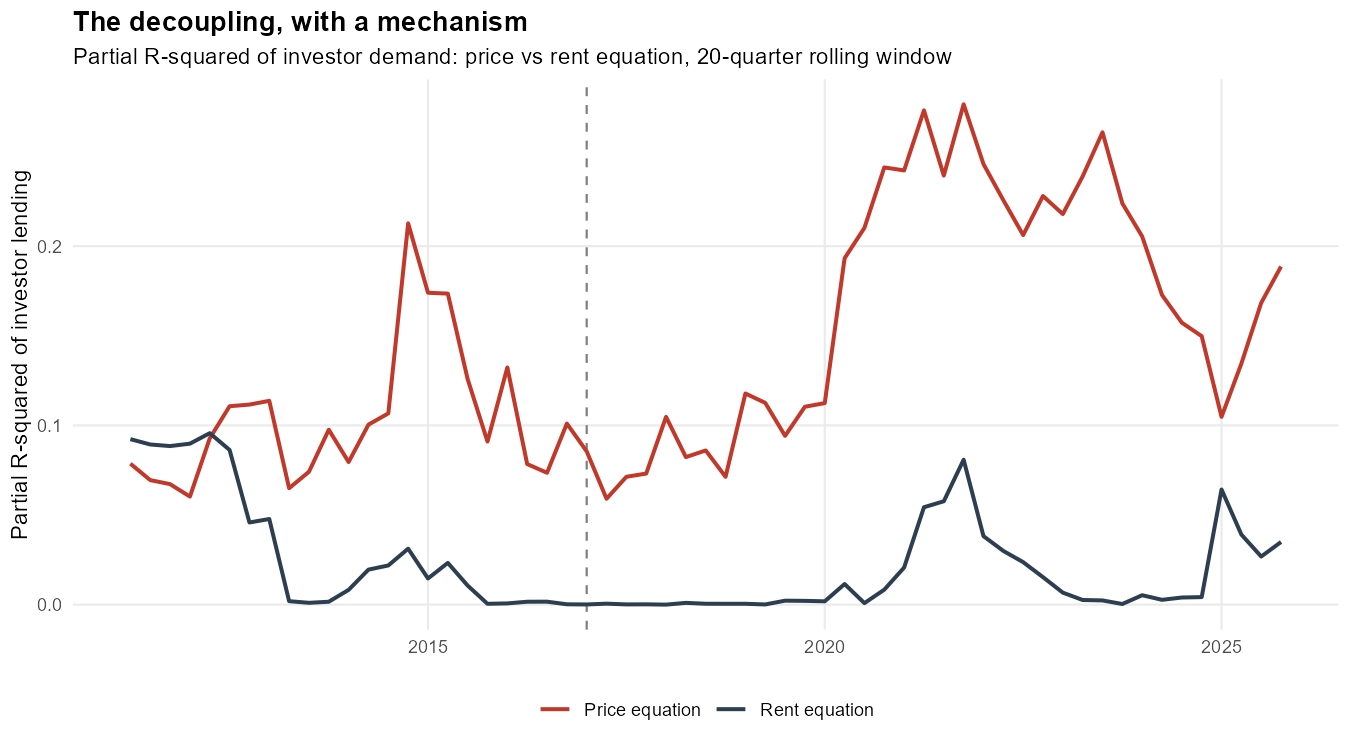
\includegraphics[width=0.8\textwidth]{fig_divergence.png}
\caption{Contemporaneous partial $R^2$ of investor credit, price
equation versus rent equation, twenty-quarter rolling window. Demoted
from the main text in favour of the local-projection evidence
(Figure~\ref{fig:lp}); reported here as a descriptive complement.}
\label{fig:rolling}
\end{figure}





\begin{table}[!h]
\centering
\caption{Overseas versus interstate migration in the rent equation:
leave-one-city-out stability}
\label{tab:mig_loo}
\begin{threeparttable}
\begin{tabular*}{\textwidth}{@{\extracolsep{\fill}}l
                S[table-format=1.4]
                S[table-format=1.4]
                S[table-format=-1.4]
                S[table-format=-1.2]@{}}
\toprule
City dropped & {Overseas} & {Interstate} & {Difference} & {$t$} \\
\midrule
None (full)  & 0.0050 & 0.0098 & -0.0048 & -2.02 \\
Sydney       & 0.0040 & 0.0113 & -0.0073 & -3.95 \\
Melbourne    & 0.0050 & 0.0114 & -0.0064 & -2.39 \\
Brisbane     & 0.0050 & 0.0103 & -0.0054 & -1.89 \\
Adelaide     & 0.0050 & 0.0101 & -0.0051 & -1.86 \\
Perth        & 0.0057 & 0.0046 &  0.0011 &  0.74 \\
\bottomrule
\end{tabular*}
\begin{tablenotes}[flushleft]
\footnotesize
\item \textit{Notes:} Each row re-estimates the rent equation with net overseas and
net interstate migration (each scaled by dwelling completions and lagged one quarter)
entered as separate regressors, dropping the named city. Columns report the two
slopes, their difference (overseas minus interstate), and the $t$-statistic on that
difference under Driscoll--Kraay standard errors. The full-sample rejection of slope
equality is not robust: it strengthens without Sydney or Melbourne, weakens below
significance without Brisbane or Adelaide, and reverses without Perth, whose interstate
slope collapses onto the overseas one. The overseas/interstate wedge is therefore a
Perth-specific feature rather than a general property of the capitals, and the omnibus
tightness numerator is adequate for the panel as a whole.
\end{tablenotes}
\end{threeparttable}
\end{table}

\begin{table}[!h]
\small
\centering
\caption{Unit Root Test Results}
\label{tab:unit_root}
\begin{threeparttable}
\begin{tabular*}{\textwidth}{@{\extracolsep{\fill}}l
S[table-format=-2.2, table-space-text-post = {***}]
S[table-format=-2.2, table-space-text-post = {***}]@{}}
\toprule
& \multicolumn{2}{c}{ADF Statistic} \\
\cmidrule(lr){2-3}
Variable & {Level} & {First Difference} \\
\midrule
Rental Price Index & -4.40\sym{***} & -14.01\sym{***} \\
Property Price Index & -3.47\sym{**} & -14.37\sym{***} \\
GFCF Public & -2.23 & -16.44\sym{***} \\
Migration & -4.18\sym{***} & -12.24\sym{***} \\
GFCF Private & -2.26 & -14.58\sym{***} \\
Housing Services Consumption & -1.42 & -13.84\sym{***} \\
Total Dwelling Completions & -2.77 & -19.72\sym{***} \\
Cash Rate & -4.77\sym{***} & -10.85\sym{***} \\
Hourly Wages & -3.95\sym{**} & -14.33\sym{***} \\
Labour Income & -1.87 & -13.98\sym{***} \\
Full-time Employment & -1.84 & -13.89\sym{***} \\
\bottomrule
\end{tabular*}
\begin{tablenotes}[flushleft]
\footnotesize
\item \textit{Notes:} ADF with constant and trend.
***\textit{p}<0.01, **\textit{p}<0.05, *\textit{p}<0.1. At the five percent
level the rental and property price indices, migration, the cash rate, and hourly
wages reject a unit root in levels, while public and private GFCF, housing services
consumption, dwelling completions, labour income, and employment do not and are
integrated of order one. Every series is stationary in first differences. This
mixture of integration orders is typical in macro-regional panels and motivates
differencing the $I(1)$ series while entering the stationary tightness ratio in
levels; we include the lagged price--rent gap as a level control rather than
imposing a cointegrating error-correction relationship, which a panel
residual test does not robustly support.
\end{tablenotes}
\end{threeparttable}
\end{table}





\end{appendices}

\end{document}